%!TEX TS-program = xelatex
%!TEX encoding = UTF-8 Unicode

% \documentclass[12pt,a4paper]{article}
\RequirePackage{tikz}

% \documentclass[sn-apacite,xelatex]{sn-jnl}
% \documentclass[smallextended]{svjour3}
\documentclass{article}

% \usepackage{program}
% \catcode`\|=12\relax

\usepackage[margin=1in]{geometry}
\usepackage[toc]{appendix}
% \usepackage{natbib}
\usepackage[backend=biber, style=apa, sortcites=false, uniquelist=false,natbib=true,doi=false,isbn=false,url=false,eprint=false,pagetracker, ibidtracker=constrict]{biblatex}
\DeclareSourcemap{
  \maps{
    \map{
      \step[fieldset=entrysubtype, null]
      \step[fieldset=address, null]
      \step[fieldset=location, null]
    }
  }
}

\addbibresource{references.bib}

% \usepackage{authblk}
% \usepackage[hyperref]{acl2020}
\usepackage[colorlinks=true,citecolor=blue]{hyperref}
% \usepackage{times}
\usepackage{textcomp}
\usepackage{textgreek}
\usepackage{latexsym}
% \usepackage{subcaption}
% \usepackage{float}

\usepackage{tikz}
% \usepackage{tikzscale}
\usepackage{pgfplots}
\usetikzlibrary{shapes,positioning,calc,arrows.meta,arrows,patterns,patterns.meta}
\usepackage{tikzscale}
\usepackage{subcaption}

\usepackage{longtable}
\usepackage{multirow}
\usepackage{multicol}

\usepackage{amsmath,bm}
\usepackage{amssymb}
% \usepackage{bbm}
\usepackage{dsfont}
% \usepackage[utf8x]{inputenc}
\usepackage{textcomp}
\usepackage{textgreek}
\usepackage[french,english]{babel}
\usepackage{latexsym}
\usepackage{url}  %Required
\usepackage{graphicx}  %Required
\frenchspacing  %Required
\usepackage{url}
\usepackage{tabularx}
\usepackage{booktabs}
\usepackage{array}
\renewcommand{\UrlFont}{\ttfamily\small}

\usepackage[acronym,nomain,nonumberlist]{glossaries}
\makeglossaries
\renewcommand*{\glsgroupskip}{}

\DeclareMathOperator*{\argmax}{arg\,max}
\DeclareMathOperator*{\argmin}{arg\,min}

\newacronym{lhc}{LHC}{Large Hadron Collider}

\newacronym{desy}{DESY}{\textit{Deutsches Elektronen-Synchrotron}}
\newacronym{slac}{SLAC}{Stanford Linear Accelerator Center}
\newacronym{cern}{CERN}{Conseil Européen de Recherche Nucléaire}

\newacronym{aps}{APS}{American Physical Society}
\newacronym{aip}{AIP}{American Institute of Physics}
\newacronym{pacs}{PACS}{Physics and Astronomy Classification Scheme\textregistered}

\newacronym{hep}{HEP}{High-Energy Physics}

\newacronym{ot}{OT}{Optimal Transport}

\title{Adapting to a changing scientific landscape: the case of high-energy physics}

\title{Specialization versus adaptation: exploring the evolution of high-energy physicists' research agenda}

% \journalname{TBD}


% \usepackage[misc]{ifsym}
\newcommand*{\affaddr}[1]{#1} 
\newcommand*{\affmark}[1][*]{\textsuperscript{#1}}

\author{Lucas Gautheron}

% \author{Lucas Gautheron \protect\affmark[1,2]}
    
% \institute{
%  Lucas Gautheron \\   \email{lucas.gautheron@gmail.com}\\ORCID: 0000-0002-3776-3373\\\\
%  \affaddr{\affmark[1]Interdisciplinary Centre for Science and Technology Studies (IZWT), University of Wuppertal, Germany}\\
%  \affaddr{\affmark[2]Sciences Po, médialab, Paris, France}
% }

\date{}

\begin{document}

\maketitle

\begin{abstract}
    
\end{abstract}

% \keywords{XXX}


% Ideas for further analyses:

% \begin{itemize}
%     \item Evaluate effect of institutinal instability (i.e. amount of successive affiliations over the period considered) on change score?
%     \item Evaluate effect of academic age?
%     \item Inspect a few profiles of interest by hand, e.g. most significant shifts from Electroweak sector to Dark matter. Maybe send out emails to these physicists and ask a few questions to understand why they have shifted to new research problems and what allowed them to do so.
% \end{itemize}

% Improvements to the model:

% \begin{itemize}
%     \item The topic distribution of papers that have lots of co-authors should contribute comparatively less to an author's intellectual capital.
%     \item Consider Horseshoe priors (at least for matrix $\gamma$) in order to handle sparsity. Strong evidence of sparsity of $\gamma$. Use \citep{Piironen2017}?
% \end{itemize}

Robustness checks:

\begin{itemize}
    \item Make sure that topics are rather autonomous: e.g., that they are strongly correlated with experiments such that those belong to typically 1 topic at most. 
    \item Make sure that conclusions not sensitive to number of publications required for each time period. Re-do analyses for different thresholds and check. Although I want to look into committed high-energy physicists, so we cannot just lower the publication threshold. Besides the effect of career stage has been considered
    % \item Compare correlation between $\log p_{\theta|w}$ and $\log p_{\theta'|w}$ (or between $\theta_{d,i}$ and $\theta_{d,j}$) with the effect of intellectual/social capital [done, not very conclusive]
\end{itemize}

Questions:

\begin{itemize}
    \item Should we add a short description of each ``research area'' in the section that introduces the topic model?
    \item Should we anonymize physicists' names when looking into individual examples? I guess we should.
\end{itemize}

Further analyses planned:
\begin{itemize}
    \item Plug ``individual knowledge'' as a covariate into the model and see what knowledge enhances certain trajectories/shifts to other research areas
    \item Look into variables that explain whether scientists expanded or shrunk their research agenda. Currently change score does differentiate between these two strategies.
    \item Look into different strategies: consolidation, expansion, migration, etc.
\end{itemize}

\section{Introduction}

Scientists are subject to conflicting incentives. On one hand, they must work within the realm of their expertise, where they can most effectively exploit their prior knowledge and compete with other experts; such a conservative preference for familiar research topics is at the root of specialization. On the other hand, scientists are simultaneously compelled to revise their research agenda and engage with increasingly promising research areas to which they might not be as acquainted, in order to benefit from more exposure, to secure more perennial funding for their work, or to seize job opportunities\footnote{Mention scientific bubbles; paper about problem choice not being about choice}. Thus, in some instances, specialization may be at odd with the need to adapt to the decay of certain research opportunities and the growth of new ones. Therefore, we may ask: how scientists navigate the trade-off between specialization and adaptation? This conflict is in some respect similar to the ``essential tension'' between ``tradition'' and ``innovation'' proposed by \citet{Kuhn1997}, or that between ``exploration'' and ``exploitation'' proposed by \citet{March1991}, which have been explored quantitatively in previous works \citep{Foster2015,Jia2017,Aleta2019,Chakresh2023}. The balance between ``specialization'' and ``adaptation'', however, must be distinguished from the balance between normal, incremental science one one side, and the risky exploration of uncharted territories on the other, which is the focus of \citet{Foster2015}. In particular, ``adaptation'' is not tantamount to innovation or disruption, for ``adaptation'' can sometimes be a conformist move (e.g. as a result of a band-wagon effect, cf. \citealt{Fujimura1988}\footnote{Cite Cyrus Mody or some relevant paper about ``scientific bubbles''?}). In fact, adaptation could very well consist in an a continued enterprise of ``normal science'' converted to new epistemic goals. In this paper, we propose to focus on what enables individuals to adapt, and which kinds of knowledge are more malleable than others. We posit that scientists' ability to adapt (and survive) within a changing epistemic environment depends primarily on two kinds of resources they can mobilize to this end, namely intellectual and social capital.  We develop a quantitative comparative approach for studying how scientists change their research agenda in response to transformations in their field, while measuring the effect of ``capital'' (``intellectual' or ``social'') on their individual trajectories. In particular, we apply the proposed model to a cohort of high-energy physicists between years 2000 and 2020.

High-energy physics is especially interesting, since the historical drivers of progress in the field -- particle accelerators -- are now being contested by emerging astrophysical experiments, such that there is a strong incentive for physicists to adapt and seize these new opportunities. And yet, at the same time, high-energy physics remains one of the most specialized subfields within physics, thus raising questions about its ability to adapt \citep{Battiston2019,Aleta2019}. Our approach reveals which kinds physicists have been more able to take the turn from ``colliders'' to ``cosmos''. It also demonstrates that scientists with more prior expertise in a domain tend to remain more specialized in this domain. Moreover, we show that having more collaborators with expertise in a target research area increases the likelihood of a physicist to redirect focus to this research area later in their career.

Our contribution has three components: i) a theoretical component, by discussing fundamental features of change in scientists' research interests; ii) a methodological dimension, through the elaboration of statistical models for studying scientists' trajectories; and finally iii) an empirical component, by documenting the case of high-energy physics.

The paper is structured as follows. In the rest of the introduction, Subsection \ref{sec:conceptual} summarises previous research and lays out the conceptual background on which rests our analysis; Subsection \ref{sec:hep} introduces the context of high-energy physics to which we apply our methodology; and Subsection \ref{sec:hypotheses} summarises the hypotheses that will be evaluated throughout the paper.

Section \ref{sec:methods} elaborates our methodology, starting with the data used in the paper (\ref{sec:data}), followed by the topic model approach for measuring the contribution of authors to each ``research area'' (\ref{sec:topics}), our measures of intellectual and social ``capital'' (\ref{sec:capital}), and, finally, our model for scientists' individual trajectories (\ref{sec:model}).

Section \ref{sec:results} then proceeds with the results of our analysis: i) the aggregate transfers of attention between research areas at the level of the community (\ref{sec:macro}); ii) the magnitude of changes in scientists' research agenda and how it is affected by capital (intellectual and social) and career stage (\ref{sec:magnitude}); iii) an exploration of interesting cases (\ref{sec:cases}). Finally, we explore the outcomes of scientists' trajectories (\ref{sec:outcomes}) as evidence for the incentives that they receive to adapt and/or the relative success of different strategies. 


\subsection{\label{sec:conceptual}Empirical and conceptual background}

Evolution in the research areas explored by scientists (in particular physicists) throughout their careers has been the focus on several previous works. For instance, by mapping the trajectories of 103,246 physicists over 26 years using the American Physical Society dataset and its topic classification (the \gls{pacs}), \citet{Aleta2019} have demonstrated that physicists usually work on different topics by the end of their career, while remaining within the same general area -- e.g., condensed matter physicists remain condensed matter physicists. They show differences across sub-fields of physics, such that ``exploitation'' (i.e. specialization, by opposition to the ``exploration'' of new topics) is especially more prevalent in particle and nuclear physics. Moreover, they show that change in research topics typically happens gradually over the years, and that scientists remain conservative in the early years of their careers. Similarly, \citet{Battiston2019} analyzed the publication record of 135,877 physicists between 1985 and 2015 and found that high-energy physicists have a comparatively low probability of contributing to other sub-fields of physics, in line with \citet{Aleta2019}'s observation. In contrast to \citet{Aleta2019}, however, \citet{Jia2017} find an exponentially decaying scientists' interest change distribution, i.e. large changes in interests throughout careers are less likely\footnote{\citet{Aleta2019} and \citet{Jia2017} used to same data, and this discrepancy could be explained by the different decisions these authors made regarding which physicists should be included in their analysis (depending on their publication counts) and which papers to include in the estimates of ``initial'' and ``final'' research areas}. \citet{Jia2017} also find that physicists tend to investigate a few core topics quite frequently, as well as many ``peripheral'' topics less frequently. They also show that physicists are more likely to investigate topics that they have recently worked on (which they call a ``recency'' effect), or topics more similar to those they have previously explored (which they call ``subject proximity''). Moreover, \citet{Jia2017} proposed different models to account for the structure of changes in research topics they observe. For instance, they show that simulations from a model in which scientists draw combinations of ideas from a topic pool that itself drifts gradually qualitatively reproduces the observed interest change distribution. In a much less recent paper, \citet{Gieryn1978} compiled data that suggested astronomers were most likely to alter their ``problem set'' -- their research agenda -- gradually, than they were to do so abruptly by switching to completely different problems altogether (what he calls ``migration''). In particular, recognizing that scientists typically investigate several research questions at the same time, \citeauthor{Gieryn1978} proposed four mechanisms of gradual change: ``accretion'' (a problem is added to the problem set),  ``selective substitution'' (one problem is replaced by another in the problem set), or ``selective disengagement'' (one problem is dropped from the problem set). All these works are very valuable for understanding the structure of changes in scientists' interests. Overall, they show that i) problem change is gradual, and that ii) it involves different scales, such that scientists can investigate different topics while remaining in the same broad research area and while preserving certain ``core interests''. However, these works do not relate changes in scientists' research agendas to changes in the epistemic and institutional context, to the incentives that scientists receive, or to the resources that they can leverage in order to broaden their research opportunities. In particular, they do not explain differences in physicists' behaviors, except in terms of their sub-field of origin or career stage. This is the gap that this paper aims to address by exploring the effect of different variables on scientists' research topics, in the context of a transforming epistemic landscape that provides incentives to adapt.  
In the following, we introduce the concepts that underlie our quantitative approach to this problem.

Our central question is: why scientists respond differently to changes in their environment over time?  In that respect, the problem of scientists' adaptation to a changing epistemic landscape can be compared to that of the adaptation of institutions under changing circumstances, and it is useful to take a little detour via the literature addressing the later question.  A key notion in this context is that of ``path-dependency'', according to which the outcome of ``previous [political] battles'' may have a lasting effect on the evolution of institutions and determine future arrangements. Path-dependency is a natural consequence of ``increasing returns'' \footnote{See \citealt{Pierson2000} for a discussion of path-dependency and increasing returns in the contexts of economics and politics.}, which designate situations where perpetuating certain options yields increasing gains, such that an early commitment to such options ``lock'' actors into perpetuating such options. Arguably, the long-lasting effects of scientists' early research topics on their career is a case of path-dependency due to ``increasing returns''. One contributing factor is the presence of \textit{large fixed costs} \citep{Pierson2000}: students must accumulate a lot of knowledge before being proficient enough to publish in a research area. Yet, in the context of historical institutionalism, it has been argued that the importance of path-dependency should not be overstated: although institutions tend to feature path-dependency, the process through which they ``survive'' over long periods of time often requires continuous change\footnote{``The language of stasis and inertia is particularly unhappy because as the world around institutions is changing their survival will not necessarily rest on the faithful reproduction of those institutions as originally constituted, but rather on their ongoing active adaptation to changes in the political and economic environment in which they are embedded.'' \citep[p.~293]{Thelen2004}}, in a way that may transgress their initial purposes or cumulatively add up to significant transformations. Similarly, although it is plausible that scientists' prior knowledge effectively constrains their opportunities and therefore later career developments (thus exhibiting some level of ``path-dependency''), it might also be that scientists' cultivation of their knowledge capital requires a sustained process of change, either by progressively re-purposing their knowledge to new ends of higher perceived epistemic or social value, by incorporating complementary bits knowledge, or by renouncing to certain ideas or methods. Such gradual moves may allow scientists to strategically retain some of  the benefits of ``problem retention'' (e.g., the exploitation of ``accumulated skills and resources'' in one area, or ``of an established research network'', p.~106) while progressively investing resources in new and promising research directions. 
%Another source of positive-feedback are \textit{learning effects}; and again, in scientific research, increased knowledge 

%As a result of these effects, the costs of moving to new research areas can be higher than the benefits of switching.


 % Although institutions also tend to feature path-dependency, whereby the outcome of ``previous [political] battles'' may have a lasting effect \citep{Thelen2004}, the process through which institutions ``survive'' over long periods of time often requires continuous change\footnote{``The language of stasis and inertia is particularly unhappy because as the world around institutions is changing their survival will not necessarily rest on the faithful reproduction of those institutions as originally constituted, but rather on their ongoing active adaptation to changes in the political and economic environment in which they are embedded'', \citep[p.~293]{Thelen2004}}. 
 % Similarly, although it is plausible that scientists' prior knowledge effectively constrains their opportunities and therefore later career developments (thus exhibiting some level of ``path-dependency''), it might also be that scientists' cultivation of their knowledge capital requires a sustained process of change, either by re-purposing their knowledge to new ends of higher perceived epistemic or social value, by incorporating complementary bits knowledge, or by abandoning certain ideas or methods.


Figure \ref{fig:research-agenda} illustrates how scientists can reshape their research agenda portfolio, e.g. for seizing new research opportunities, while taking advantage of their own prior knowledge base as much possible. It represents the research agenda of a scientist in two separate time-periods, in terms of the resources they utilize and to what research areas these resources are applied. Resources are to be understood broadly: they might be concepts, models, methods, or technical skills mastered by a researcher. Problem areas are designated by different colors. A resource can be simultaneously applied to different ends, as expressed by the hatched rectangles; however, resources are frequently tailored and fit for specific research areas. Scientists can take advantage of their prior knowledge in different ways. They can of course embrace specialization and keep pursuing the same kind of problems with the same theoretical and methodological tools.  Alternatively, they may apply their prior knowledge to new purposes; this is akin to what \citet{schon1963displacement} calls ``concept displacement'' and such a strategy can be leveraged to enter new research areas \citep{Mulkay1974}. We call it ``conversion'', in reference to the typology of incremental change proposed by \citet{mahoney_thelen_2009} in the context of historical institutionalism. Of course, not all intellectual or methodological resources can be successfully applied to new research areas. We expect that certain transitions from one problem area to another are more likely than others; in fact, it is plausible that scientists are more likely to shift resources and attention to research areas that are less ``distant'' to their previous expertise. Overall, we expect that scientists build up as much as possible on their prior knowledge, which is their best asset, thereby reinforcing the continuity in the evolution of their research agenda.

It is likely, however, that building upon prior knowledge is insufficient for adaptation. As illustrated in Figure \ref{fig:research-agenda}, entering new research areas usually  requires ``layering'' (here again, borrowing the terminology from historical institutionalism), i.e. the introduction of new concepts, models, or methods, ontop of other resources. Yet, acquiring new knowledge and skills comes at a cost. In practice, scientists may avoid some of these extra costs by collaborating with researchers that already have expertise in the target domain. This, arguably, is easier and more natural for scientists that already have connections with scientists previously established in the target research area. We therefore expect that such scientists will more often redirect their attention to research areas in which a lot of their collaborators have expertise.

\begin{figure}
    \centering
    \begin{tikzpicture}
    % First Stack
    \foreach \i in {1,2,3}
        \draw [fill=blue!20] (0,{(\i-1)*0.5}) rectangle (3,{\i*0.5}) node[pos=.5] {Resource \i};

    \foreach \i in {4,5}
        \draw [fill=red!25] (0,{(\i-1)*0.5}) rectangle (3,{\i*0.5}) node[pos=.5] {Resource \i};

    \draw [preaction={fill=green!30},pattern={Lines[angle=-45, line width=3mm]}, pattern color=red!25] (0,{(6-1)*0.5}) rectangle (3,{6*0.5}) node[pos=.5] {Resource 6};

    \foreach \i in {7,8}
        \draw [preaction={fill=green!30},pattern={Lines[angle=-45, line width=3mm]}, pattern color=red!25] (0,{(\i-1)*0.5}) rectangle (3,{\i*0.5}) node[pos=.5] {Resource \i};
        
    % Arrow between stacks
    \draw [->, dashed] (3.25,1.25) -- (5.75,1.25) node[midway, above] {Conversion};
    % \draw [->, dashed] (3.5,2.75) -- (5.5,2.75) node[midway, below] {Displacement};
    \draw [->, dashed] (3.25,3.25) -- (5.75,3.25) node[midway, above] {Conversion};

    \draw [->, dashed] (3.25,{8.5*0.5}) -- (5.75,{8.5*0.5}) node[midway, above] {Layering};

    \draw [->, dashed] (4.25,{8.5*0.5}) -- (5.75,{7.5*0.5});
    
    % Second Stack
    
    \foreach \i in {1,2}
        \draw [fill=blue!20] (6,{(\i-1)*0.5}) rectangle (9,{\i*0.5}) node[pos=.5] {Resource \i};

    \foreach \i in {3,4,5}
        \draw [fill=red!25] (6,{(\i-1)*0.5}) rectangle (9,{\i*0.5}) node[pos=.5] {Resource \i};

    \draw [fill=red!25] (6,{(6-1)*0.5}) rectangle (9,{6*0.5}) node[pos=.5] {Resource X};

    \draw [fill=yellow!20] (6,{(7-1)*0.5}) rectangle (9,{7*0.5}) node[pos=.5] {Resource 7};

    \draw [fill=yellow!20] (6,{(8-1)*0.5}) rectangle (9,{8*0.5}) node[pos=.5] {Resource Y};

    \draw [fill=yellow!20] (6,{(9-1)*0.5}) rectangle (9,{9*0.5}) node[pos=.5] {Resource Z};
    
    % \draw [fill=red!20] (5,{(1-1)*0.5}) rectangle (8,{1*0.5}) node[pos=.5] {Concept A};
    % \draw [fill=red!20] (5,{(2-1)*0.5}) rectangle (8,{2*0.5}) node[pos=.5] {Concept B};
    % \draw [fill=red!20] (5,{(3-1)*0.5}) rectangle (8,{3*0.5}) node[pos=.5] {Concept C};
    % \draw [fill=red!20] (5,{(4-1)*0.5}) rectangle (8,{4*0.5}) node[pos=.5] {Concept D};

    % \node (a) at (1.5,5) {2000 to 2009};
    % \node (b) at (7.5,5) {2015 to 2019};
    
    \end{tikzpicture} 

    \caption{Schematic illustration of the changes in a scientist' ``research portfolio'' over time. Each color represents a different ``problem area''. Resources are any intellectual or methodological assets that a scientist uses to address scientific problems from each research area.}
    \label{fig:research-agenda}
\end{figure}


We have discussed two resources that scientists can leverage to navigate the trade-off between specialization and adaptation. The first is their own prior expertise, which enables them to compete in research areas where these intellectual resources are either necessary or scarce and relevant\footnote{One of the sources mention works in HEP that show physicists sometimes run away from too competitive areas}. The second is the expertise to which they potentially have access via their social network. We propose to view both these resources as ``capital'' \citep{Bourdieu1986} that can be leveraged in a changing epistemic landscape, where boundaries across specializations must be crossed. Bourdieu's ``capital'' designates assets of different kinds that individuals (e.g. scientists) can accumulate and leverage in the competitive context of their field. It is indeed ``capital''  (whether ``economic'', ``cultural'', ``social'' or even ``symbolic'', cf. \citealt{Bourdieu1986}) that defines the scope of scientists' opportunities, and therefore their ability to broaden their research agenda. In this paper, we will consider two kinds of capital: the cultural capital possessed by scientists in the form of scientific knowledge (which we will refer to as ``intellectual capital''), and social capital. We will propose measures that operationalize these concepts in a way relevant for our study and evaluate their effect on the magnitude of transfers of attention across research areas. Although the notion of capital may provide an account of what defines the scope of scientists' opportunities, it is not sufficient to explain why physicists take certain turns or not. For that it is also necessary to understand the incentives that actors receive, and how crucial it is to them to respond to these incentives. Consequently, we will also compare the outcomes -- in terms of scientific credit -- of physicists, depending on whether they took certain turns to growing research areas or cultivated their specialization instead. We will also evaluate the effect of career stage on migrations, given that the need to respond to changes in the epistemic and institutional environment is presumably different for early-career physicists than it is for tenured professors and researchers.


Before introducing our data and our quantitative approach, we briefly discuss recent developments in high-energy physics and our motivations for applying our approach to this subfield of physics. 

% For instance, in a case-study, \citet{Mulkay1974} discusses the role of ``concept displacement'' in the migration of radio-astronomers to new research communities. 



\subsection{\label{sec:hep}The case of high-energy physics: navigating a changing epistemic landscape}

Historically, the field of particle physics has relied on experimental input from larger and larger particle colliders in order to achieve progress. Such efforts have culminated in 2010 with the start of the Large Hadron Collider (LHC), the largest particle accelerator ever built, involving about 10,000 collaborators. However, the LHC has found no evidence for anything that was not already predicted by the Standard Model of particle physics, and it is increasingly plausible that in fact no conceivable particle accelerator would ever find any evidence for new particles or phenomena, resulting in a ``crisis'' in particle physics \citep{susy_crisis}. Although the \gls{lhc} will continue taking data for years, and plans for a successor are being discussed, some have even speculated that particle physics as we know it had come to an end \citep{Harlander2023,Kosyakov2023}, ``the proscenium
[being] captured by astrophysics and cosmology'' instead \citep{Kosyakov2023}. What does this mean for high-energy physics? In a recent assessment of the state of the field, physicist Mikhail Shifman claimed that ``pause in accelerator programs we are witnessing now is not necessarily [\dots] the end of explorations at short distances [at high energies]''; instead, such explorations ``will continue, perhaps in a new form, with novel devices, and at a different pace'' \citep{Shifman2020}.

In the meantime, new experimental opportunities have indeed emerged. The era of Gravitational Waves astronomy has begun in 2016, with the announcement of the first ``direct'' detection of such waves from a black-hole merger by LIGO \citep{Abbott2016}. Highly sensitive direct searches of dark matter of astrophysical origin, with the LUX and Xenon experiments, are another example of these new experimental opportunities that may provide access to phenomenal domains relevant to high-energy physics that would be otherwise inaccessible in accelerators\footnote{Dark matter can be detected in particle colliders as missing energy but only to the extent that it can be produced in collisions of visible matter particles.}. These transformations in the landscape of experimental opportunities in high-energy physics can be visualized in Figure \ref{fig:experiments}. This Figure shows the share of citations received by the most cited experiments in high-energy physics. It shows the dominance of the Large Hadron Collider in accelerator-based research, as well as the emergence of probes of astrophysical phenomena, both of which can be traced back to around 2010. Another phenomenon of interest the declining interest in neutrino experiments since the early 2000s, especially in experiments studying non-astrophysical neutrinos\footnote{The Super-Kamiokande experiment and the Sudbury Neutrino Observatory found conclusive evidence for neutrino oscillations in 1998 and 2001 respectively. Takaaki Kajita and Arthur B. McDonald were awarded the 2015 Nobel Prize in Physics for these discoveries (\url{https://www.nobelprize.org/uploads/2017/09/advanced-physicsprize2015.pdf}).}. More signs of the declining power of collider physics and the perceived promise of astrophysical experiments in \gls{hep} can be found in the changes in the ``trading zone'' in high-energy physics: astrophysics seem to replace collider physics in the exchanges of knowledge between experimentally inclined phenomenologists and more mathematically inclined theorists \citep{Gautheron2023}.

\begin{figure}
    \centering
    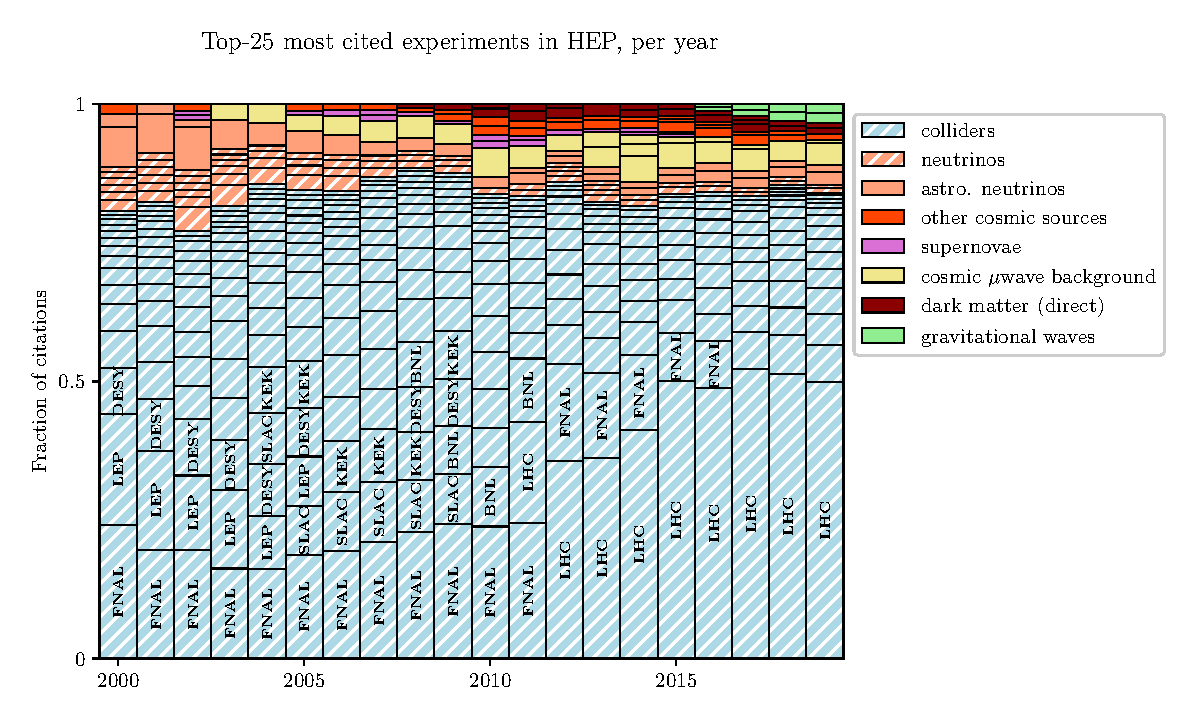
\includegraphics[width=\textwidth]{plots/experiments.eps}
    \caption{Share of citations of each of the most cited experiments in high-energy physics literature, between 2000 and 2019. Hatched rectangles correspond to experiments observing particles produced in colliders or nuclear reactors; other rectangles correspond to observations of phenomena or particles of astrophysical origin. We use citation and experiment data from the Inspire HEP database \citep{InspireAPI}. The classification of these experiments is our own. }
    \label{fig:experiments}
\end{figure}


What have been the consequences of a such a reshaping of the landscape of research opportunities on problem choice in high-energy physics? In what follows, we propose to investigate how high-energy physicists have adapted in reaction to these changes in the first two decades of the 21st century. In doing so, we aim to explore the contribution of different factors that may have affected the trajectories of individual physicists: what explains why certain physicists have moved on to other topics, while others have pursued similar interests instead? 


\subsection{\label{sec:hypotheses}Hypotheses}

We propose to make our hypotheses more explicit by formulating them into statements amenable to statistical testing. Our guiding hypotheses will be:


\begin{itemize}
    \item[\textbf{H1}] There is a growing interest in astrophysics among high-energy physicists.
    \item[\textbf{H2}] Diverse intellectual capital broadens scientists' research opportunities:
    \begin{itemize}
        \item[\textbf{H2a}] Scientists with more diverse intellectual capital tend to change their research agenda more.
        \item[\textbf{H2b}] Scientists with more expertise in certain research areas more likely to commit further resources to these research areas.
    \end{itemize}
    \item[\textbf{H3}] Diverse social capital broadens scientists' research opportunities:
    \begin{itemize}
        \item[\textbf{H3a}] Scientists with more diverse social capital tend to change their research agenda more.
        \item[\textbf{H3b}] Scientists with more collaborators tend to change their research agenda more
        \item[\textbf{H3c}] Scientists with more access to intellectual resources in certain research areas via their collaborators are more likely to commit further resources to these research areas.
    \end{itemize}
    \item[\textbf{H4}] Career stage has an effect on physicists' tendency to change their research agenda:
    \begin{itemize}
        \item[\textbf{H4a}] Scientists with tenured/stable positions change their research agenda more (e.g. because they have more ability to choose their research topics or to take risks).
        \item[\textbf{H4b}] Scientists with tenured/stable positions are more conservative toward their research agenda (e.g. because they have less incentives/pressure to change it).
    \end{itemize}
    \item[\textbf{H5}] Physicists who committed to high-energy astrophysics in the late 2010s have received more scientific credit compared to the others
\end{itemize}

Note that our approach will also be exploratory. Beyond hypothesis testing, we aim to unveil transfers of knowledge across research areas in high-energy physics without any assumption about what these transfers might be; in fact, we will employ unsupervised methods (with no training labels) in order to segment the field into distinct research areas, thus leaving the room open for surprises.

% \begin{itemize}
%     \item H1: physicists change their research agenda gradually
%     \item H2: it is most natural to switch from one research area to another if they already are associated in the literature
%     \item H3: positive effect of social capital
% \end{itemize}

% TODO: better grounding in i) Bourdieu's notion of capital and ii) the contemporary literature..

% \begin{itemize}
%     \item H1: physicists with higher abilities to establish new collaborations (higher social capital) are more likely to switch to new topics.
%     \item H2: physicists with more prestigious institutional affiliations (higher symbolic capital) have been more likely to invest new topics.
%     \item H3: physicists with more ``credit'' (higher h-index) have a higher chance to invest new topics
%     \item H4: physicists can invest new topics more easily if they have collaborators with expertise in these topics.
%     \item H5: physicists with a more diverse expertise have more ability to invest new topics.
% \end{itemize}

\section{\label{sec:methods}Methods}

\subsection{\label{sec:data}Data}

Our source of data is the Inspire HEP database \citep{InspireAPI}. It aggregates high-energy physics literature from a variety of sources, including main scientific publishers and arXiv.org, and has been used in a number of previous works \citep{Perovi2016,Strumia2021,Sikimi2022,Gautheron2023}. This database is in free-access and includes a variety of high-quality data: semantic data about each paper (mainly their title and abstract, sometimes also keywords and \gls{pacs} categories), curated authorship and institutional affiliations, lists of references and experiments associated to each paper. However, full-texts are not directly provided, although most of them could in theory be retrieved from arXiv.org, where physicists usually upload their work prior to publication.

In our analysis, we include all papers from the categories ``Theory-HEP'' and ``Phenomenology-HEP'' (according to the classification of the database which is itself based on that of the arXiv), to which most  high-energy physics publications belong. Of course, this excludes the minority of purely experimental high-energy physics publications. Patterns of specialization among experimenters would be interesting to study as well; however, experimental papers are typically authored by thousands of collaborators, most of whom were not actually involved in most publications, and authorship data brings no information about individual physicists' specialization. Nevertheless, considering theoretical and phenomenological publications still allows us to investigate how theorists and phenomenologists have adapted to the changes outline above. In total, the corpus includes $D=186,162$ papers published between 2000 and 2019, the time-range that is covered in our analysis. 

For the cohort analysis, we consider two time-periods. The initial phase (2000-2009) is used to infer the initial ``research agenda'' of each physicist of the cohort as well as their social capital. The later phase (2015-2019) is used to measure how each physicist's research agenda has shifted from the first period to the second period, in response to the changes outlined above. We only include physicists with at least 5 publications during each time-period (2000 to 2009, and 2015 to 2019), resulting in a cohort of 1930 physicists. As a result, our study is limited to physicists that have remained dedicated to high-energy physics enough to have published that many papers during each phase. In other words, what we measure are the physicists' strategies for adapting (and ``surviving'') \textit{within} high-energy physics. 

At this one must emphasizes a critical challenge when using bibliometric databases for analyzing scientists' careers, namely the confusion of authors\footnote{Add references}, due to either authors with identical names being mistaken with one another, or authors with names spelled in different ways (e.g. R.~Feynman instead of Richard Feynman) incorrectly identified as several individuals. The Inspire HEP database is particularly helpful in that respect, as it implements both automatized and manual measures for the disambiguation of author names\footnote{``INSPIRE	 uses	 advanced	
algorithms	 to	 try	 to	 deduce	if	 “Richard	 Feynman”	is	 the	 same	 person indicated	 on	 an	
article	 as	 “R	 Feynman”,	 “RP	 Feynman”,	 and	 so	 on. [\dots] Since	 these	 routines	 can	 never	 be	 perfect,	 the	
author	profile	pages	contain	a	link	(“This	is	me…”)	to	an	interface	where	researchers	can	
unambiguously	verify	their	publications	list	on	INSPIRE (“paper	claiming”).	This	insures	
that	 the	publications	are	assigned	 to	 their	personal	name	persistently. In	 the	past	 two	
years	 the	 INSPIRE	 team	 has	invited	 researchers	 via	 email	 to	 use	 this	 tool	 and	 correct	
their	publication	profiles	on	 INSPIRE.	Within	the	 first	year,	response	rates	were	rather	
high,	on	average	about 40\%''. (``Background	information	on	the	INSPIRE	website'', June 2014, \url{https://twiki.cern.ch/twiki/pub/Inspire/WebHome/INSPIRE_background.pdf})} -- authors are given the opportunity to correct their records, and they have an incentive to do so. For instance, this has allowed \citet{Strumia2021} to use these data in order to analyze gender gaps in physicists' research careers. Nevertheless, occasional mis-identifications remain possible. 

\subsection{\label{sec:topics}Clustering the literature}

The first step is to evaluate how much attention physicists have devoted to each research area during each time-period. In contrast to \citet{Jia2017,Battiston2019,Aleta2019}, we do not rely on \gls{pacs} categories to map research areas: such data are only sparsely available within our corpus of \gls{hep} literature, and this would make this approach inapplicable to contexts other than physics. Instead, research areas are extracted through the use of a topic model, which simultaneously recovers latent ``topics'' within the corpus and their vocabulary distributions.  Given research areas should be rather broad and autononomous, we perform a coarse-grained classification of the literature into only $K=20$ ``topics''. One could consider a finer-grained classification, and there is always some level of arbitrariness involved in choosing the amount of topics. This is not as much an issue of topic models themselves: as \citet{Gieryn1978} puts it, ``in such analyses [of problem change], empirical findings will in part reflect the defined scope of problem areas'', which is itself arbitrary. In fact, that topic models give some control over the cognitive scale to be considered can be considered a feature, rather than a bug.

In order to perform the clustering task, we use the \gls{etm} developed by \citealt{Dieng2020}, which relies on pre-trained embeddings representations of the keywords. This model provides more reliable classifications of heavy-tailed vocabulary distributions\footnote{For rarely occurring keywords, meaning can be better inferred by taking advantage of their proximity with other keywords within documents, which 
is precisely the kind of information that word-embeddings encode. Traditional topic models dismiss all information about the relative position of keywords.}, which is especially important in our case, since we seek accurate estimates of the amount of keywords in each abstract that belong to each ``topic''. We train the model on the whole corpus (all $D=186,162$ documents published between 2000 and 2019). Keywords are extracted from the papers' titles and abstracts by filtering n-grams between one and three words matching certain syntactic expressions that we can expect to carry scientific information (by designating concepts, models, methds etc.), following the procedure described in \citealt{Gautheron2023} and \citealt{omodei_tel-01097702}. Keywords' embeddings are learned using a skip-grap model in a 50 dimension space (few dimensions are needed given the small size of the vocabulary, $V=4,751$). In the end, we obtain the topics listed in table \ref{table:research_areas}. This table shows their most-frequent keywords, as well as the \gls{pacs} categories that are most correlated with them, for purposes of validation. Of the 20 resulting topics, 16 topics are interpretable; the other four seem to regroup keywords that do not clearly refer to any specific research area (e.g. ``paper, approach''). As is apparent in the table, these four topics correlate poorly with the \gls{pacs} categories, thus confirming their lack of scientific dimension. As a result, we exclude them from the rest of the present analysis, and we only consider the remaining $K=16$ topics that actually designate research areas.

The next step is to go through all papers and estimate to what extent they contribute to each research area. In the \gls{etm} -- as in topic models in general--, documents are mixtures of several topics; moreover, keywords may belong to several topics. This is a desirable feature, because certain concepts have different meanings or functions depending on the context, and some concepts do not clearly belong to any research area. More importantly, this is crucial to our approach, insofar we must be sensitive to situations in which scientists have repurposed certain concepts to new research goals; i.e., instances where the same resources are applied in a new context (a new research area). The variational inference algorithm in \citet{Dieng2020} marginalises out the topic of each word occurrence during training. In order to recover the topic associated with each occurrence of a word, we first evaluate the probability $P(z_{di}=k|w_{di},\bm{\theta}_{d})$ that keyword $i$ in document $d$ belongs to each topic $k$, given $\bm{\theta}_d$, the topic distribution of $d$. We then assign the most probable value to $z_{di}$:

\begin{equation}
    z_{di} := \argmax_{k=1,\dots,K} P(z_{di}=k|w_{di},\bm{\theta}_{d}) =  \argmax_{k=1,\dots,K} \dfrac{P(w_{di}|z_{di}=k)P(z_{di}=k|\bm{\theta}_d)}{P(w_{di}|\bm{\theta}_d)}
\end{equation}

This allows us to exploit the context $\bm{\theta}_d$ while inferring the topic (research area) as part of which each keyword (each resource) has occurred. In the process, we discard ambiguous keywords for which $H(z_{di})\geq \log{2}$, where $H$ denotes the entropy of the distribution $P(z_{di}=k|w_{di})$. Either such keywords do not carry any scientific content, or the context is insufficient to disambiguate among the possible research areas to which they might belong\footnote{Idea: show examples of keywords with low entropy and keywords with high entropy.}.

From the values $z_{di}$, we can then recover $X_{a,k}$, the amount of times resources (concepts, models, methods, etc.) in papers (co-)authored by $a$ were applied in the context of a research area $k$ in the initial time-period (2000 to 2009). Mathematically, $X_{a,k}=\sum_{d\in P,a\in A_d} \sum_i \delta(z_{di},k)$, where $A_d$ is the set of authors of a publication $d$, and $P$ is the set of papers published between 2000 and 2009, and $\delta$ is the Kronecker delta. We then compute a matrix $Y_{a,k}$ using the same procedure, based on publications from the later time-period (2015 to 2019) this time. Finally, from this we define the normalized distributions $x_{ak} \equiv X_{ak}/\sum_{k'} X_{ak'}$ and $y_{ak} \equiv Y_{ak}/\sum_{k'} Y_{ak'}$. They represent how each scientist $a$ divided their attention across research areas during each time-period.

\subsection{\label{sec:capital}Measuring capital}

We aim to evaluate the effect of two resources on scientists' trajectories, namely intellectual and social capital \citep{Bourdieu1986}, as they can be ``measured'' from bibliometric data. An extensive review of the usage of Bourdieu's notion of capital in bibliometrics has been provided by \citet[p.~198-200]{Schirone2023}, with most references addressing symbolic and social capital and none focusing on cultural capital. 

\subsubsection{Intellectual capital}

We propose to represent intellectual capital by a vector $\bm{I_a}=(I_{ak})$ that purportedly measures the proficiency of an author $a$ in each research area $\k \in \{1,\dots,K\}$. We construct it in a way similar to $\bm{x_{a}}$, summing the contribution of keywords dedicated to each research area in the publications of each author during years 2000 to 2009. However, this time, we weigh publications differently depending on their amount of authors; indeed, intuitively, publications with fewer co-authors convey more information about each author's own expertise. Mathematically, we apply a weight $1 \over |A_d|$, where $|A_d|$ is the amount of authors of publication $d$\footnote{A justification for this weight is that, in a publication with $n$ authors, the probability that any one of them has been responsible for introducing any particular concept or method present in the paper is $\mathcal{O}(1/n)$. }:

\begin{equation}
    I_{ak} \propto  \sum_{d\in P,a\in A_d} \dfrac{1}{|A_d|}\sum_i \delta(z_{di},k)
\end{equation}

The vector $\bm{I_a}$ is normalized, such that $\sum_k I_{ak}=1$; as a result, $\bm{I_a}$ only captures the distribution of knowledge among research instead of the ``absolute magnitude'' of knowledge in each area. This could be justified by asserting that physicists all saturate their cognitive capacities such that the magnitude of their ``total knowledge'' is roughly identical, and that the main difference between them is how they choose to divide their cognitive resources across epistemic domains (for instance, by specializing in one single domain or more). Of course, other measures could in principle be proposed and plugged into the model. 

\subsubsection{Social capital}

A variety of quantitative measures of social capital have been proposed in the context of scientific research \citep{Abbasi2014,Schirone2023}, and their relative relevance must be assessed depending on the phenomenon under investigation. The simplest measure of social capital is the amount of collaborators of a scientist (which amounts to degree centrality in the co-authorship network). More sophisticated weighted variants, that take into consideration the frequency of collaborations, have also been suggested \citep{Abbasi2014}. Other measures are related to the notion of betweeness centrality, which concerns the extent to which an actor ``bridges'' a network. For instance, \citet{BurtBrokerage2007} has proposed to measure social capital in term of brokerage, i.e. the ability of an individual to overcome gaps (``structural holes'') in a social network. In a co-authorship network, for example, scientists with high brokerage are involved in many collaborations that gather scientists who would otherwise have no ties with each other. The distinction between these different measures is important; in some cases, for instance, it is detrimental to have many redundant contacts, therefore brokerage may be more beneficial than the sheer amount of contacts. \citet{Abbasi2014} distinguishes two general approaches to social capital, depending on whether the emphasis is put on ``power'' versus ``diversity''. They also propose their own measures based on the distribution of scientists' collaborators performance -- as evaluated by their h-index -- and show that these measures correlate better with scientists' performance (i.e. their h-index or citation count). All of the measures discussed by \citet{Abbasi2014} are scalars, i.e. they represent social capital as a single number, that is derived from the co-authorship network and sometimes other data (e.g. citations). However, one single number necessarily misses multiple dimensions of social capital, some of which cannot even be captured by social networks alone \citep{MartnAlczar2019}. In the following, we propose instead to focus on one aspect of social capital, that is, ``social-intellectual'' capital. We propose to represent it by a vector that encodes how much cognitive resources can be leveraged by scientists \textit{within each} research area by mobilizing their network.

According to \citet{Bourdieu1980}, ``the volume of social capital possessed by a particular agent [\dots] depends on the extent of the network of links that he can effectively mobilize, and on the volume of capital (economic, cultural or symbolic) possessed by each of those to whom he is linked''. In that respect, social capital can have multiple dimensions, and one must decide which is more relevant depending on the context. We are especially interested in ``social-intellectual'' capital, i.e., how much expertise a scientist $a$ has access to (in a given research area) via their collaborators, which we will represent as a vector $\bf{S}_{a}$. It is a function of i) how many collaborators a scientist has -- as inferred from the co-authorship network --, ii) the strength of these collaborations, and iii) how much expertise each of their collaborators holds in each research area. Therefore, we propose to measure the social-intellectual capital $\bf{S}_{a}$ of $a$ as the sum of the intellectual capital of their collaborators, weighted by the strength of their relationship:

\begin{equation}
    \bm{S}_{a} \equiv \sum_{c \in \text{co-authors}(a)} w_{ac} \bm{I}_{c|a}
\end{equation}

The vector $\bm{I}_{c|a}$ is the intellectual capital of $c$, evaluated by excluding papers they co-authored with $a$ (in order to further disentangle the effect of an author's own intellectual capital and intellectual capital available to him in social form). The weight $w_{ac}$, which represents the strength of the relationship between $a$ and $c$, is defined as:

\begin{equation}
    w_{ac} \equiv \max_{d, \{a,c\} \subset A_d} \frac{1}{|A_d|-1}
    \label{eq:weighing_scheme}
\end{equation}

Where $d$ runs over all publications and $A_d$ is the set of the co-authors of a paper $d$. Such a weighing scheme, inspired from \citealt{Newman2004} (eq. 4), captures the fact that a paper with, say, two co-authors, signals a stronger relationship between the authors than a publication with a dozen authors.\footnote{There are different ways to derive such an expression, starting from different assumptions about the division of labor within collaborations. For instance, we may assume that in a collaboration, each author interacts with a constant amount of co-authors in practice (regardless of the total amount of co-authors); in that case, that the probability that they interact with one specific co-author in particular is $\propto \frac{1}{|A_d|-1}$. We may alternatively assume that authors interact with all their co-authors, but that since they devote a constant amount of time to the collaboration, the average time spent with each co-author is, again, $\propto \frac{1}{|A_d|-1}$.} It must be emphasized that Equation \eqref{eq:weighing_scheme}, however, does not take into account the relative frequency of each collaboration, and old collaborations count just as much as recent ones.

\subsubsection{Diversity and magnitude of capital}

We have proposed two constructs ($\bm{I_a}$ and $\bm{S_a}$) operationalizing the notions of intellectual and social capital. Although these are vectors (with one dimension per research area), scalar metrics of potential relevance can be readily derived from these constructs. For instance, one can calculate the exponential of the Shannon entropy their distribution (resp. $D(\bm{I_a})=\exp{H(\bm{I_a})}$ and $D(\bm{S_a})=\exp{H (\bm{S_a})}$). Such measures express the \textit{diversity} of a scientist capital. They are maximal when resources are distributed evenly across research areas, and minimal when all resources are located within a single research area. We can also derive measures of the \textit{magnitude} of social capital $M(\bm{S_a})$, for instance $M(\bm{S_a})=\log{(1+\sum_k S_{ak})}$ -- here, the logarithm conveys that gains from going from, say, 50 collaborators to 51 collaborators are much lesser than the benefits of going from, say, three to four collaborators. Figure \ref{fig:capital_measures} shows the Pearson correlation between these measures, plus a measure of brokerage\footnote{We evaluated brokerage as the amount of pairs of scientists that have collaborated with a given physicist while having no common collaborator except for this physicist. This effectively measures the extent to which this physicist connects otherwise disconnected scientists.}, as evaluated on the cohort of high-energy physicists. Intellectual diversity and social diversity are strongly correlated. Brokerage and the magnitude of social capital (which is similar to degree centrality) are even more correlated; a potential explanation is that strongly connected scientists (with high degree centrality) are also those scientists who initiate collaborations between otherwise disconnected scientist (which is what brokerage captures); nevertheless, brokerage is better correlated to diversity than sheer magnitude, as could be expected. Presumably, which dimension of capital (e.g., ``diversity'' or ``power'', per \citealt{Abbasi2014}) matters more depends on the criterion of performance under investigation, and must be assessed empirically.

\begin{figure}
    \centering
    \includegraphics[width=0.8\textwidth]{plots/capital_measures.eps}
    \caption{Correlation between different measures of capital.}
    \label{fig:capital_measures}
\end{figure}

\subsection{\label{sec:model}Modelling trajectories}

In order to model the physicists' trajectories, we propose a hierarchical multinomial--logistic normal model inspired from the multinomial-dirichlet model for ecological inference by \citet{RosJiaKin01}. Figure \ref{fig:ei} illustrates the intuition underlying this model. It is assumed that how a scientist divides his attention across research areas at a later stage of their career ($\bm{Y_{a}}$) is a function of how they divided their attention initially ($\bm{X_{a}}$); this captures the features of problem change illustrated in Figure \ref{fig:research-agenda}, according to which change in agenda typically involves transfers of knowledge from one research area to another. A more formal representation of the model is given in Figure \ref{fig:model_structure}. It shows that $\bm{Y_{a}}$ is a function of the previous research agenda ($\bm{X_{a}}$), and of a mixing matrix $\theta_a$ that measures the extent to which attention has been re-distributed to different research areas. The matrix $\theta_a$ is drawn from a hierarchical process, thus capturing the ``average'' behavior of the cohort. $\theta_a$ is also a function of co-variates ($\bm{Z_a}$ in Figure \ref{fig:model_structure}), in our case intellectual and social capital, which are supposed to affect how individuals have revised their research agenda. Of course, one could consider the effect of many other covariates; for instance, the effect of holding specific bits of knowledge (models, methods, etc.).

Formally speaking, we assume that $\bm{Y_{a}}$ derives from a multinomial process involving linear combinations of $(X_{ak})$:

\begin{equation}
    \bm{Y_a} \sim \text{multinomial}(\sum_{k=1}^{K} x_{ak}\theta_{ak1} ,\dots,\sum_{k=1}^{K}x_{ak}\theta_{akK})
\end{equation}

Where $\theta_{akk'}$ is the fraction of attention to a topic $k$ that has been redirected to a topic $k'$. %All that is observed are the variables ($\bm{X_{a}}$) and ($\bm{Y_{a}}$) (and co-variates such as intellectual and social capital); however, $\theta$ can be inferred by leveraging the correlations between the attention devoted to a given research area in the initial phase and in the later phase: so is the power of ecological inference\footnote{A paradigmatic use-case of ecological inference is the estimation of voting trajectories. In this case, $\bm{X_a}$ and $\bm{Y_a}$ would be the votes registered for different candidates at two different elections at each precinct, and $\theta_{akk'}$ would be the fraction of voters from precinct $a$ having voted $k$ at the first election and $k'$ at the later election.}. 
Moreover, we introduce intellectual capital $\bm{I_a}$ and social-intellectual capital $\bm{S_a}$ as covariates for transfers $\theta$ in the model, through a generalized linear model:

\begin{equation}
    \bm{\theta_{ak}} = \text{softmax}\left(\beta_{ak1} + \gamma_{k1} I_{a1} + \delta_{k1} S_{a1}, \dots,\beta_{akK} + \gamma_{kK} I_{aK} + \delta_{kK} S_{aK}\right)
    \label{eq:glm}
\end{equation}

In this expression, $\delta_{k,k'}$ is the effect of the expertise in $k$ (social capital) that is available through the scientists' collaborators on the magnitude of their shift in attention from $k$ to $k'$. Similarly, $\gamma_{kk'}$ is the effect of having more expertise in $k'$ (intellectual capital) on shifting attention from research area $k$ toward research area $k'$. For instance, high values of $\gamma_{kk}$ (the diagonal elements of $\gamma$) would imply that physicists are more conservative toward research areas in which they have comparatively more expertise. The coefficients $\beta_{akk'}$ encode the average behavior of the cohort plus individual deviations to the average behavior that are unexplained by the covariates. Finally, the priors for this hierarchical model are:

\begin{align}
    \beta_{akk'} &\sim \mathcal{N}(\mu_{k k'},\sigma_{k k'}) \text{ for } 1\leq k' \leq K-1 \text{ and } \beta_{ak K} = 0\\
    \mu_{k k'} &\sim \mathcal{N}(\alpha \delta_{kk'},1)\\
    \delta_{k,k'},\gamma_{k,k'} &\sim \mathcal{N}(0,1) 
\end{align}

Where the matrix $\mu$ encodes the ``average'' behavior. In order to fit the model to the data, we use Stan's Hamiltonian Monte-Carlo sampler. At this stage, it is important to emphasize a weakness of models of ecological inference, that is, their weak identifiability. Weak identifiability arises when the data can only weakly inform certain parameters of a model \citep{Gimenez2009}. This warrants some caution when using a model such as ours for studying specific individuals (e.g. by inspecting values of $\bm{\theta_{ak}}$ for one individual); the main interest of the model lies in its ability to capture the average effect of certain covariates (e.g. social capital). This weakness converges with the criticism of ecological inference raised by the ``ecological fallacy'' argument \citep{freedman1999ecological} according to which they are limits to what can be inferred about individuals based on aggregate data. Nevertheless, our approach i) allows to estimate the average effect of certain variables on transitions between research areas and ii) the Bayesian formulation naturally accounts for the uncertainty associated with limited identifiability.


% \begin{itemize}
%     \item $\bm{X_a} = (X_{ak})$: occurrences of concepts from topic k in the initial period (2000-2004) in author's $a$ papers
%     \item $\bm{Y_a} = (Y_{ak})$: occurrences of concepts from topic k in the final period (2015-2019) in author's $a$ papers
%     \item $\bm{S_a} = (S_{ak})$ social-intellectual capital of $a$ along each topic
%     \item $\bm{x_a} = (X_{ak}/\sum_{k'} X_{ak'})$ specialization of $a$ in each topic (fraction of concepts devoted to each topic)
%     \item $\delta_{k,k'}$: effect of the expertise in $k'$ that is available through the scientists' collaborators on the magnitude of their shift in attention from $k$ to $k'$
% \end{itemize}

% \begin{align}
%     \bf{N^F_{a}} &\sim \text{multinomial}(\sum_{k=1}^{K} \frac{N^I_{ak}}{N_a}\theta_{ak1} ,\dots,\sum_{k=1}^{K}\frac{ N^I_{ak}}{N_a}\theta_{akK})\\
%     \bm{\theta_{ak}} &= \text{softmax}\left(\beta_{ak1} + \sum_i \delta^i_{ak1} x^i_{ak1}, \dots,\beta_{akK} + \sum_i \delta^i_{akK} x^i_{akK}\right)\\
%     \bm{\beta_{ak}} &\sim \mathcal{N}(\bm{\mu_k},I_K)\\
%     \mu_{k,1\leq k'<K} &\sim \mathcal{N}(0,1)\\
%     \mu_{k,K} &= 0
% \end{align}

    \tikzstyle{block} = [draw,minimum size=2em, minimum width=3em]
    \tikzstyle{block1} = [block,fill=blue!20]
    \tikzstyle{block2} = [block,fill=red!20]
    \tikzstyle{block3} = [block,fill=green!20]
    \tikzstyle{block4} = [block,fill=cyan!20]
    \tikzstyle{block5} = [block,fill=gray!20]
    \tikzstyle{block6} = [block,fill=yellow!20]
    
    \tikzstyle{pre} = []
    \tikzstyle{post} = []
    \tikzstyle{traj} = []
    \tikzstyle{pre2} = []
    \tikzstyle{post2} = []
    \tikzstyle{traj2} = []
    \tikzstyle{pre3} = []
    \tikzstyle{post3} = []
    \tikzstyle{traj3} = []
 \begin{figure}
 \centering
     \begin{subfigure}[b]{0.30\textwidth}
          \centering
          \resizebox{0.8\linewidth}{!}{
          
\begin{tikzpicture}[>=latex',baseline={(0,0)}]

    % Draw blocks, inputs and outputs
    \foreach \y in {1,2,3} {
        \node[block\y,pre] at (2,-\y) (input\y) {$X_{a,\y}$};
        \node[block\y,post] at (6,-\y) (output\y) {$Y_{a,\y}$};;
    }
    \node[block5,pre] at (2,-4) (input5) {\dots};
    \node[block5,post] at (6,-4) (output5) {\dots};
    \node[block6,pre] at (2,-5) (input6) {$X_{a,K}$};
    \node[block6,post] at (6,-5) (output6) {$Y_{a,K}$};
        \foreach \x in {1,2,3} {
        \draw[->,traj] (input1.east) -- (output\x.west) node[midway,above=-0.2em,sloped] {$\theta_{a,1,\x}$};
    }
    \draw[->,traj] (input1.east) -- (output5.west) node[midway,above=-0.2em,sloped] {$\theta_{a,1,\dots}$};
    \draw[->,traj] (input1.east) -- (output6.west) node[midway,above=-0.2em,sloped] {$\theta_{a,1,K}$};

    % \node[visible on=<1>, align=center] at (2,0.75) {Distribution\\ of attention\\ prior to\\ the LHC };

    % \node[visible on=<2>, align=center] at (6,0.75) {Distribution\\ of attention\\after\\ the LHC};

    % \path (input1) -- coordinate (branch) (block1);
    \tikzstyle{s}=[shift={(0mm,\radius)}]
\end{tikzpicture}

          }  
          % \caption{Caption A}
          % \label{fig:A}
     \end{subfigure}
     \begin{subfigure}[b]{0.30\textwidth}
          \centering
          \resizebox{0.8\linewidth}{!}{
          
\begin{tikzpicture}[>=latex',baseline={(0,0)}]

    % Draw blocks, inputs and outputs
    \foreach \y in {1,2,3} {
        \node[block\y,pre2] at (2,-\y) (input\y) {$X_{a,\y}$};
        \node[block\y,post2] at (6,-\y) (output\y) {$Y_{a,\y}$};;
    }
    \node[block5,pre2] at (2,-4) (input5) {\dots};
    \node[block5,post2] at (6,-4) (output5) {\dots};
    \node[block6,pre2] at (2,-5) (input6) {$X_{a,K}$};
    \node[block6,post2] at (6,-5) (output6) {$Y_{a,K}$};

    \foreach \x in {1,2,3} {
        \draw[->,traj2] (input2.east) -- (output\x.west) node[midway,above=-0.2em,sloped] {$\theta_{a,2,\x}$};
    }
    \draw[->,traj2] (input2.east) -- (output5.west) node[midway,above=-0.2em,sloped] {$\theta_{a,2,\dots}$};
    \draw[->,traj2] (input2.east) -- (output6.west) node[midway,above=-0.2em,sloped] {$\theta_{a,2,K}$};

    \tikzstyle{s}=[shift={(0mm,\radius)}]
\end{tikzpicture}
          }  
          % \caption{Caption B}
          % \label{fig:B}
     \end{subfigure}
     \begin{subfigure}[b]{0.30\textwidth}
          \centering
          \resizebox{0.8\linewidth}{!}{
          
\begin{tikzpicture}[>=latex',baseline={(0,0)}]

    % Draw blocks, inputs and outputs
    \foreach \y in {1,2,3} {
        \node[block\y,pre3] at (2,-\y) (input\y) {$X_{a,\y}$};
        \node[block\y,post3] at (6,-\y) (output\y) {$Y_{a,\y}$};;
    }
    \node[block5,pre3] at (2,-4) (input5) {\dots};
    \node[block5,post3] at (6,-4) (output5) {\dots};
    \node[block6,pre3] at (2,-5) (input6) {$X_{a,K}$};
    \node[block6,post3] at (6,-5) (output6) {$Y_{a,K}$};
    
    \foreach \x in {1,2,3} {
        \draw[->,traj3] (input3.east) -- (output\x.west) node[midway,above=-0.2em,sloped] {$\theta_{a,3,\x}$};
    }
    \draw[->,traj3] (input3.east) -- (output5.west) node[midway,above=-0.2em,sloped] {$\theta_{a,3,\dots}$};
    \draw[->,traj3] (input3.east) -- (output6.west) node[midway,above=-0.2em,sloped] {$\theta_{a,3,K}$};

    \tikzstyle{s}=[shift={(0mm,\radius)}]
\end{tikzpicture}
          }  
          % \caption{Caption C}
          % \label{fig:C}
     \end{subfigure}
     \caption{\textbf{Schematic representation of physicists' transfers of attention across research areas.} Each $\bm{\theta_{ak}}=(\theta_{akk'})$ represents the fraction of the attention devoted by an author $a$ to a topic $k$ (prior to the start of the LHC) that has been redirected to topics $k' \in \{1,\dots,K\}$. Therefore, $\sum_k' \theta_{akk'}=1$. For conservative that preserve exactly the same balance of research interests, $\theta_{akk'}=\delta_{kk'}$. For most physicists, however, we expect that some transfers across topics must have occurred.}
     \label{fig:ei}
 \end{figure}


\begin{figure}
    \centering
    \begin{tikzpicture}[
    node distance=1.45cm,
    obs/.style={circle,draw,fill=gray!20,inner sep=1pt,minimum size=24pt},
    latent/.style={circle,draw,color=black,inner sep=1pt, minimum size=24pt}
    ]
        \node [obs](X)  {$\bm{X_a}$};
        \node [obs](Y) [right of=X] {$\bm{Y_a}$};
        \node [latent](theta) [above of=Y] {$\theta_a$};
        \node [latent](beta) [above of=theta] {$\beta_a$};
        \node [latent](mu) [above of=beta] {$\mu,\Sigma$};
        \node [obs](cov) [left of=theta] {$\bm{Z_a}$};
        \draw [->] (X) edge (Y);
        \draw [->] (theta) edge (Y);
        \draw [->] (beta) edge (theta);
        \draw [->] (mu) edge (beta);
        \draw [->] (cov) edge (theta);
        % \draw [->] (v3) edge (v2);
        % \draw [->] (v4) edge (v3);
        % \draw [->] (v0) edge (v5);
        % \draw [->] (v6) edge (v1);
\end{tikzpicture}
    \caption{\textbf{Directed acyclic graph representation of the hierarchical model}. $\bm{X_a}$ and $\bm{Y_a}$ is the distribution of scientists $a$'s interests across research areas in the early phase and the late phase respectively. $\theta_a$ is the mixing matrix that represents how scientists $a$ shifted their attention from one research area to another. $\theta_a$ depends on a number of co-variates $\bm{Z_a}$ (e.g. $\bm{I_a}$ and $\bm{S_a}$, intellectual and social ``capital''). Observed variables are represented in gray, latent variables in white.}
    \label{fig:model_structure}
\end{figure}

 \section{\label{sec:results}Results}

 \subsection{\label{sec:macro}Macroscopic trends}

Our model can first unveil the trajectories from one research area to another at the macroscopic level, as shown in Figure \ref{fig:sankey}. In this diagram, the width of each flow is proportional to $\sum_a X_{ak}\theta_{akk'}$ (summing over each author $a$), thus directly measuring how much attention was transferred from $k$ to $k'$ at the level of the whole community. The most obvious feature is the overall conservatism of physicists toward their research areas, in other words specialization (see Table \ref{table:most_conservative}, Appendix \ref{appendix:macro}). Another feature is the growth of certain research areas, most notably ``Black holes'' and ``Dark matter''. This is in line with what was hypothesized in our introduction, as years 2010 to 2020 have seen the emergence of new probes of the cosmos, and with our hypothesis \textbf{H1} that ``there is a growing interest in astrophysics among high-energy physicists''. In the mean time, certain research areas have decayed; in particular, ``Neutrinos and flavor physics'' have considerably shrunk, as was already suggested in Figure \ref{fig:experiments} which showed the decreasing impact of neutrino experiments. On the theoretical side, ``String theory and supergravity'' has also gathered significantly less attention. The macroscopic trends unveiled by the model are also able to explain how exactly certain research areas have grown and to the detriment of which. For instance, the increasing interest in Dark matter seems to be mainly fueled by a shift away from ``Neutrinos and flavor physics'' and ``Electroweak sector''. Similarly, the growth in the interest for AdS/CFT as well as Black holes has happened at the expense of the dedication to ``String theory and supergravity'' research. Interestingly, this provides some credence to physicist Peter Woit's assessment that ``string theorists'' are no longer doing string theory per se, though they keep identifying themselves as string theorists.\footnote{As Peter Woit puts it, citing the 2022 ``Strings'' conference: ``one thing that stands out is that the string theory community has almost completely stopped doing string theory.''; and, ``[presentations' titles] make very clear what the string theory community has found to replace string theory: black holes'' (Woit, 2022, \url{https://www.math.columbia.edu/~woit/wordpress/?p=12981}); See also Woit, 2023 ( \url{https://www.math.columbia.edu/~woit/wordpress/?p=12401})} 

 \begin{figure}
     \centering
     \includegraphics[width=\textwidth]{plots/sankey_control.pdf}
     \caption{\textbf{Aggregate transfers of attention across research areas, between 2000-2009 (to the left) and 2015-2019 (to the right)}. Widths of flows are proportional to $\sum_a X_{ak}\theta_{akk'}$. Insignificant transfers (that happen less than expected by chance alone assuming random mixing) are transparent. }
     \label{fig:sankey}
 \end{figure}



% How to explain the size of individual effects? Figure \ref{fig:social-capital-distance} shows the relationship between the effect of social capital on trajectories $k\to k'$ ($\delta_{kk'}$) and the proximity of pairs of topics. The proximity of topics, calculated as the normalized pointwise mutual information between document-topic distributions, is to be roughly understood as the probability for a pair of topics to be associated within a scientific publication. We find a (modest) negative correlation ($R=-0.4$), suggesting that having collaborators with expertise in the target research area is more advantageous when the target area is more remote to one's original expertise. In other words, social capital does help overcome the effects of specialization.


% \begin{figure}
%     \centering
%     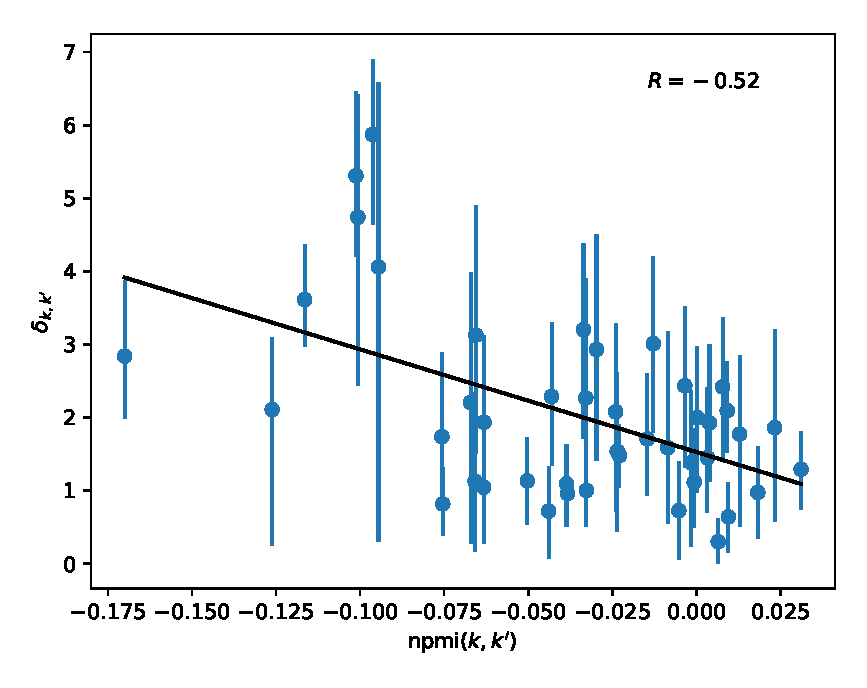
\includegraphics[width=0.8\textwidth]{plots/ei_delta_kl_dist.eps}
%     \caption{Relationship between the strength of he effect of social-capital on transfers between two research areas  (y-axis) and the proximity of these research areas (x-axis). Proximity of research areas $k$ and $k'$ is evaluated as the normalized pointwise mutual information (npmi) of $\theta_{d,k}$ and $\theta_{d,k'}$ across documents, which encodes how often these topics are combined within scientific papers.}
%     \label{fig:social-capital-distance}
% \end{figure}

\subsection{\label{sec:magnitude}Quantifying change and the effect of capital}

Whether individual scientists have remained  conservative toward their research agenda, or have instead significantly revised their priorities, can now be quantitatively measured. To this end, we propose a change score $c_a$ defined for each physicists $c_a$ as the total variation distance between their initial and late research agendas:

\begin{equation}
    c_a \equiv \mathrm{d}_{\text{TV}}(\bm{x_a},\bm{y_a}) = \frac{1}{2} \sum_k |y_{ak}-x_{ak}|
\end{equation}

This score measures how much the research agenda of a scientist has changed between the two time-periods. It is comprised between 0 (implying that research attention has remained identically distributed) and 1 (implying that the research agenda has changed entirely). The distribution of $c_a$ across authors is given in Figure \ref{fig:change_scores}. Following \citet{Gieryn1978}, we hypothesized that problem change was indeed more often gradual than an abrupt ``migration'' from one research area to another. Figure \ref{fig:change_scores}, shows that indeed, large values are quite rare. However, one must be cautious about interpreting the absolute value of $c_a$. As pointed out by \citet{Gieryn1978}, the extent to which problem change is ``gradual'' depends on the choice of ``cognitive scope'' (the broadness of research areas) and the duration of the time-periods under consideration.  Moreover, we always expect some level of fluctuations in the measured agendas, due to noise imputable to the topic model approach for measuring the contribution to each research area.

\begin{figure}
    \centering
        \includegraphics[width=0.8\textwidth]{plots/change_score.eps}
    \caption{\textbf{Distribution of change scores in the cohort}. Higher values correspond to more drastic changes in a scientists' research agenda.}    
    \label{fig:change_scores}
\end{figure}

Nevertheless, the change score allows for comparison between physicists. What explains differences in individual strategies? We propose to evaluate the role of several factors, namely: i) the diversity of intellectual capital $D(\bm{I_a})$, based on the Shannon entropy of $\bm{I_a}$; ii) the diversity of social capital $D(\bm{S_a})$, measured in a similar way; and iii) the magnitude of social capital, measured as $\log(1+\sum_k S_{ak})$. We also consider iv) the effect of career stage, which we represent as a binary variable $s_a$ such that $s_a=1$ if scientist $a$ has an affiliation that spans the whole time-period from 2000 to 2019 and 0 otherwise -- i.e. a stable/tenured position. We perform a Beta-logistic regression of $c_a$ as a function of these four variables, controlling for $Z_a=\argmax_{k} x_{ak}$, i.e. physicists' primary research area over the years 2000 to 2009. Results are shown in Figure \ref{fig:change_score_effect}.

As can be seen on this Figure, the diversity of intellectual capital has a significant positive effect. Physicists with resources in many areas indeed have more opportunities to revise their research agenda. There is also evidence of a positive effect of diversity of social capital on the magnitude of changes in scientists' research focus. The sheer magnitude of social capital, however, contributes negatively when diversity is taken into account. Presumably ``power'' (of which the amount of collaborators is a proxy) allows physicists to remain more conservative while ``diversity'' promotes change. It is notable that these dimensions of social capital can have opposite effects. Moreover, career stage has a significant effect as well: physicists with more stable positions are more conservative toward their research agenda. This could be because they have lower incentive to ``adapt'' by committing to trending research problems. It might also be that changes in host-institution are often associated with changes in research topics.

Only three research areas have a ``significant'' (95\% CL) effect, namely ``String theory \& supergravity'', ``Neutrinos and flavor physics'' (positive effect) and ``Collider physics'' (negative effect). Unsurprisingly, both of the research areas that are significantly associated with higher migration scores \textit{ceteris paribus} have shrunk significantly. that  In the case of ``Collider physics'', although the effect is barely significant in the regression (which means the effect is not particularly strong \textit{ceteris paribus}, for given values of capital and career stage), physicists whose primary category is Collider physics are by far the most conservative, with an average change score 22\% lower than that the average of high-energy physicists. It is plausible that the long time-scales of collider experiments and the specialized knowledge that they require provide stable opportunities to physicists expert in that kind of physics (as previously emphasized by \citealt[p.~138]{galison1987how}), thus encouraging further specialization.

\begin{figure}
    \centering
    \includegraphics[width=0.8\textwidth]{plots/change_score_effects.eps}
    \caption{\textbf{Effect of standardized measures of intellectual and social capital, and of career stage on the amplitude of changes in high-energy physicists' interests (as measured by the change score $c_a$)}. Diversity is evaluated in terms of the exponential of the Shannon entropy of the distribution of intellectual and social resources physicists possess across research areas. The effect of the primary research area during the initial period (2000-2009) was also included as a controlling factor. Three research areas have a ``significant'' (95\% CL) effect. Error bars indicate 95\% credible intervals. $R^2=0.15$.}
    \label{fig:change_score_effect}
\end{figure}

All these results must be interpreted with caution, considering the low variance explained ($R^2=0.15$). Nevertheless, diversity of intellectual resources seems to matter, and it is useful to look into the detail of how intellectual capital (as represented by $\bm{I_a}$, the proficiency of researchers in each aresearch area) affects trajectories. For that, we use the model introduced in Section \ref{sec:model}. In this model, the effect of intellectual diversity is directly measured by the diagonal coefficients of the $\gamma$ matrix that measure the effect of having intellectual resources in a certain area into further committing to this area. The matrix is shown in Figure \ref{fig:intellectual-capital-effect}. Most coefficients on the diagonal are significantly greater than zero, thus suggesting that physicists with a strong specialization in a research area have a higher tendency to consolidate their specialization in this area. Several explanations can be suggested. One of them is that having more expertise in an area gives physicists an advantage over their ``competitors'' that they seek to exploit as much as possible. Another explanation might be that being specialized into one area makes it harder to seize opportunities in other areas.

\begin{figure}
    \centering
    \includegraphics[width=0.8\textwidth]{plots/ei_gamma_control.eps}
    \caption{Effect of intellectual capital (expertise possessed by each physicist) on the magnitude of transfers of attention from one research area to another. Rows represent research areas of origin and columns represent target research areas. Stars represent statistical significance ($\ast$: 95\%; $\ast\ast$: 99\%).}
    \label{fig:intellectual-capital-effect}
\end{figure}

Similarly, the effect of social-intellectual capital on transfers from one research area to another, given by the matrix $\delta_{kk'}$ (see equation \ref{eq:glm}), is shown in Figure \ref{fig:social-capital-effect}. As it appears in this figure, statistically significant effects are always positive. This implies that having many collaborators with expertise in a target area generally increases the likelihood of redirecting attention toward this area, as hypothesized. 


\begin{figure}
    \centering
    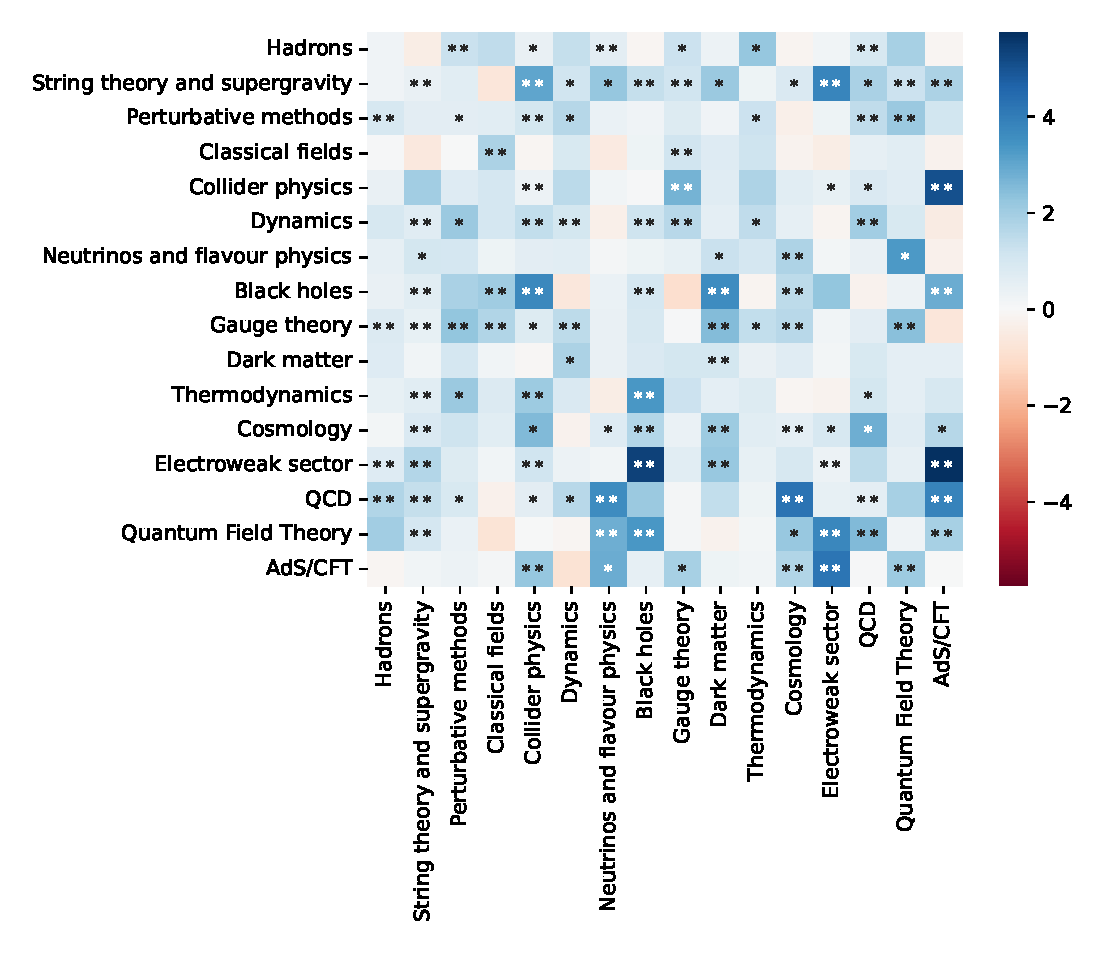
\includegraphics[width=0.8\textwidth]{plots/ei_delta_control.eps}
    \caption{Effect of social-intellectual capital (expertise accessible through one's collaborators) on the magnitude of transfers of attention from one research area to another. Rows represent research areas of origin and columns represent target research areas. Stars represent statistical significance ($\ast$: 95\%; $\ast\ast$: 99\%).}
    \label{fig:social-capital-effect}
\end{figure}

It must be highlighted that the change score $c_a$ gives no indication about the way the research agenda of a scientist has changed. For instance, two very opposite strategies may contribute to high values of $c_a$. On one hand, one can diversify their research agenda through the investigation of new research areas, or through a more even balance of research focus; we might call such strategies ``diversification''. On the other hand, one can narrow down their research portfolio, by deserting certain research areas and concentrating increasingly on one or a few topics (which we might call ``consolidation''). Scientists' tendency toward diversification can be measured by computing the difference between the effective amount of research areas explored in the second and the first time-periods. Mathematically, we define a diversification score $\Delta_a$ as:

\begin{equation}
    \Delta_a \equiv D(\bm{y_a})-D(\bm{x_a})
\end{equation}

Where $D$ again denotes the exponential of the Shannon entropy, which is a good measure of diversity\footnote{The Shannon entropy of the discrete uniform distribution on $\{1,\dots,n\}$ (of probability mass-function $(1/n,\dots,1/n)$) is $\log{n}$, such as that the exponential of the entropy is roughly the effective amount of outcomes for the distribution ($n$).}. High values indicate diversification, while negative values indicate consolidation. The absolute values of $\Delta_a$ are not so interesting given that they depend on factors such as the duration of each time-period; for instance, since the second time-period is shorter, the average value of $\Delta_a$ is negative. Nevertheless, this metric allows for comparisons between scientists and for the evaluation of the effect of a number of variable on the choice between diversification and increased specialization. The effect of capital and career stage on the diversification score is shown in Figure \ref{fig:diversification_score_effect}. In contrast to the magnitude of change, the diversity of intellectual capital now has a negative effect. This might seem paradoxical; however, intellectual capital basically measures one's prior research diversity, and it is difficult further diversify an already highly diversified research. On the other hand, the diversity of social capital (i.e., of intellectual resources available via one's connections) still contributes positively, although the evidence is quite low. This suggests that entering new research areas is somewhat easier when one has access to diverse expertise via their network. Career stage has no  noticeable effect on diversification. Two research areas seem to have a positive effect (String theory \& supergravity and Quantum Field Theory), both of which are very theoretical. ``Collider physics'' still has a strong negative effect, probably for the reasons outlined above. More interestingly, ``Dark matter'' has a negative effect which could be explained by the fact scientists with prior commitment to this research area had less incentive to diversify their research portfolio and more incentive to focus increasingly on this topic given its increasing success over the following  years.
 
\begin{figure}
    \centering
    \includegraphics[width=0.8\textwidth]{plots/diversification_score_effects.eps}
    \caption{\textbf{Standardized effects of capital and career stage on the diversification of high-energy physicists' interests (as measured by the diversification score $\Delta_a$)}. $R^2=0.24$.}
    \label{fig:diversification_score_effect}
\end{figure}

\subsection{\label{sec:cases}Exploring individual careers}

It is insightful to look into scientists at both extremes of the distribution of change scores from Figure \ref{fig:change_scores}. To this end, we selected the 20 physicists with the lowest and the highest change scores, as shown in Tables \ref{table:low_change} and \ref{table:top_change}. 
In both these tables, the change score ($c_a$) is complemented with measures of the diversity of each physicist's intellectual capital ($\exp D(\bm{I_a})$) and social-intellectual capital ($\exp D(\bm{S_a}$)) defined as the exponential of the Shannon entropy of these vectors (thus expressing the effective amount of research areas in which physicists have resources).


The first table shows the physicists that have conserved their initial research agenda the most. Strikingly, 15 out of 20 are specialized in ``Collider physics'', in line with our observation that this particular research area is more conservative and specialized. ``Neutrinos and flavor physics'' occurs several times as well. This might seem contradicting with our finding that this research area is associated with higher change scores. However, Neutrinos physics are still a significant research area and many physicists must have remained committed to it. For instance, S.~Goswami's started her career in the late 1990s, working on neutrinos oscillations \footnote{\url{https://en.wikipedia.org/wiki/Srubabati_Goswami}} and has remained dedicated to this research area after what she describes as the ``golden age'' of neutrino physics (i.e. the early 2000s, \footnote{\url{https://www.ias.ac.in/public/Resources/Initiatives/Women_in_Science/Contributors/srubabati.pdf}}).
%Moreover, although the investigation of the ``Electroweak sector'' has mostly relied on particle accelerators, it is noteworthy that physicists specialized in the former research area have more effectively taken the turn to the investigation of Dark matter. This suggests that converting knowledge of the phenomenology of the the electroweak sector to the study of dark matter is easier than re-adapting knowledge specific to particle accelerators to this end. 

Table \ref{table:top_change} shows the 20 physicists with the highest change scores.  Looking into the share of attention dedicated by each scientist to each area, one can see that high change scores are usually reached, unsurprisingly, when physicists exit a research area and enter a new one in which they had almost no prior interest. %There is one exception: physicist M.~A.~Luty is shown to have a high change score, and yet his principal research area has remained identical. In this case, the change score is presumably high because this physicist has abandoned several research areas to which he previously contributed, to focus instead on physics of the Electroweak sector. In other words, this physicist has \textit{consolidated} his prior specialization into one research area, by ``disengaging'' \citep{Gieryn1978} from other commitments.

In order to make sure that these cases of high migration were not false positives due to the failure to properly disambiguate authors, we have inspected each of them manually, by comparing physicists' Inspire HEP profiles with data from their personal websites, as well as their university or LinkedIn profiles. We found that only one of them to be a false positive due to failing author disambiguation, namely ``T.~Fuchs'', i.e. the author with the highest change score. All other cases are accurate.
%For instance, physicist M.~Redi can be seen to have moved away from Quantum gravity research toward the investigation of Dark matter. And indeed, his personal web-page reads: ``I have worked in several different fields of theoretical physics from extra-dimensional theories to supersymmetry and modifications of gravity. My main interest at the moment is phenomenology but I keep interests in more formal subjects such us strongly coupled dynamics [\dots] I am currently mostly working on cosmology, dark matter theories and gravitational waves'' \footnote{\url{https://sites.google.com/site/redi76/research}, accessed on 11/10/2023}.
For instance, on G.~Ferretti's university webpage, one can read: ``Gabriele Ferretti joined Chalmers in 1999. For the first ten years he has been mainly involved in research in quantum field theory and string theory with emphasis on their formal aspects. Since the start of the LHC he has also become interested in phenomenological applications of quantum field theory and model building'' \footnote{\url{https://www.chalmers.se/en/persons/ferretti/}, accessed on 11/10/2023}.
%In the case of Bin.~Wu, interestingly, the model has successfully captured his shift to Collider physics, even though most  keywords in his publications have remained consistent\footnote{\url{https://inspirehep.net/authors/983139}}. This suggests our approach is able to detect the research area to which certain knowledge is being applied (e.g. fundamental \gls{qcd} vs \gls{qcd} applied to the physics of hadron colliders). Upon closer inspection, however, S.~D.~Katz's change score is overstated due to early publications focusing on \gls{qcd} being incorrectly classified as not belonging to Phenomenology-HEP.

Comparing tables \ref{table:low_change} and \ref{table:top_change}, one can see that physicists with high change scores tend to have much more diverse expertise (intellectual capital) and collaborators (social-intellectual capital). In other words, such physicists have had more opportunities to adapt or revise their research agenda. This is in line with our previous result.

\begin{table}[H]
\centering
\caption{Physicists with the lowest change scores $c_a$. $D(\bm{I_a})$ and $D(\bm{S_a})$ measure the diversity of intellectual and social capital. Numbers in parentheses indicate the share of attention dedicated to each research area. Asterisks ($\ast$) indicate physicists with a permanent position.}
\label{table:low_change}
\begin{tabular}{p{0.15\textwidth}|c|c|c|b{0.25\textwidth}|b{0.25\textwidth}}
\toprule
              Physicist & $c_a$ & $D(\bm{I_a})$ & $D(\bm{S_a})$ &                   Previous main area &                       Current main area \\
\midrule
     J.~Huston ($\ast$) &  0.04 &          2.96 &          5.50 &              Collider physics (0.61) &              Collider physics (0.60)\\ \hline
  U.~D.~Alesio ($\ast$) &  0.05 &          1.68 &          4.50 &              Collider physics (0.87) &              Collider physics (0.88)\\ \hline
            S.~Schumann &  0.06 &          4.15 &          7.90 &              Collider physics (0.46) &              Collider physics (0.45)\\ \hline
          A.~V.~Lipatov &  0.06 &          2.88 &          4.28 &              Collider physics (0.68) &              Collider physics (0.68)\\ \hline
           Andreas Metz &  0.06 &          2.01 &          3.61 &              Collider physics (0.85) &              Collider physics (0.89)\\ \hline
               I.~Vitev &  0.07 &          2.95 &          5.49 &              Collider physics (0.72) &              Collider physics (0.73)\\ \hline
 Xin Nian Wang ($\ast$) &  0.07 &          2.61 &          4.06 &              Collider physics (0.77) &              Collider physics (0.75)\\ \hline
             S.~Goswami &  0.07 &          2.15 &          5.22 &  Neutrinos \& flavour physics (0.83) &  Neutrinos \& flavour physics (0.79)\\ \hline
         Y.~Mehtar Tani &  0.07 &          2.75 &          5.17 &              Collider physics (0.75) &              Collider physics (0.75)\\ \hline
           M.~Trigiante &  0.07 &          5.11 &          6.42 & String theory \& supergravity (0.55) & String theory \& supergravity (0.56)\\ \hline
     F.~Murgia ($\ast$) &  0.07 &          1.84 &          4.57 &              Collider physics (0.86) &              Collider physics (0.87)\\ \hline
     B.~Kayser ($\ast$) &  0.07 &          2.07 &          4.94 &  Neutrinos \& flavour physics (0.76) &  Neutrinos \& flavour physics (0.77)\\ \hline
   J.~F.~Owens ($\ast$) &  0.07 &          2.01 &          5.42 &              Collider physics (0.78) &              Collider physics (0.80)\\ \hline
           A.~Bacchetta &  0.07 &          2.07 &          3.19 &              Collider physics (0.84) &              Collider physics (0.81)\\ \hline
P.~M.~Nadolsky ($\ast$) &  0.07 &          3.19 &          5.28 &              Collider physics (0.62) &              Collider physics (0.59)\\ \hline
            D.~Martelli &  0.07 &          4.42 &          5.97 & String theory \& supergravity (0.57) & String theory \& supergravity (0.58)\\ \hline
              C.~Pisano &  0.08 &          1.77 &          4.53 &              Collider physics (0.87) &              Collider physics (0.88)\\ \hline
   M.~Strikman ($\ast$) &  0.08 &          2.77 &          4.99 &              Collider physics (0.77) &              Collider physics (0.75)\\ \hline
    J.~Nemchik ($\ast$) &  0.08 &          2.67 &          4.69 &              Collider physics (0.80) &              Collider physics (0.78)\\ \hline
Zhi Zhong Xing ($\ast$) &  0.08 &          3.44 &          8.17 &  Neutrinos \& flavour physics (0.71) &  Neutrinos \& flavour physics (0.65)\\ \hline
\bottomrule
\end{tabular}
\end{table}

\begin{table}
\centering
\caption{Physicists with the highest change scores $c_a$. $D(\bm{I_a})$ and $D(\bm{S_a})$ measure the diversity of intellectual and social capital. Numbers in parentheses indicate the share of attention dedicated to each research area during each time-period. Asterisks ($\ast$) indicate physicists with a permanent position.}
\label{table:top_change}
\begin{tabular}{p{0.15\textwidth}|c|c|c|b{0.25\textwidth}|b{0.25\textwidth}}
\toprule
              Physicist & $c_a$ & $D(\bm{I_a})$ & $D(\bm{S_a})$ &                            Previous main area &                               Current main area \\
\midrule
                T.Fuchs &  0.93 &          4.38 &          6.50 &                           QCD (0.53$\to$0.00) & Neutrinos \& flavour physics (0.00$\to$0.64)\\ \hline
   N.G.Sanchez ($\ast$) &  0.88 &          7.52 &         13.08 &                   Black holes (0.37$\to$0.03) &                  Dark matter (0.00$\to$0.57)\\ \hline
   V.V.Braguta ($\ast$) &  0.88 &          5.03 &          8.04 &                       Hadrons (0.45$\to$0.00) &                          QCD (0.05$\to$0.60)\\ \hline
   G.B.Cleaver ($\ast$) &  0.83 &          6.34 &         12.22 & String theory \& supergravity (0.40$\to$0.00) &                    Cosmology (0.03$\to$0.62)\\ \hline
      J.Martin Camalich &  0.82 &          2.34 &          4.57 &                           QCD (0.78$\to$0.03) &                      Hadrons (0.06$\to$0.38)\\ \hline
Kwei Chou Yang ($\ast$) &  0.81 &          3.58 &          7.80 &                       Hadrons (0.63$\to$0.03) &                  Dark matter (0.00$\to$0.78)\\ \hline
      S.D.Katz ($\ast$) &  0.80 &          6.50 &         10.85 &                   Dark matter (0.42$\to$0.03) &                          QCD (0.06$\to$0.47)\\ \hline
    G.Ferretti ($\ast$) &  0.78 &          5.22 &          6.18 & String theory \& supergravity (0.52$\to$0.00) &           Electroweak sector (0.01$\to$0.58)\\ \hline
         K.Bhattacharya &  0.78 &         10.79 &         10.59 &  Neutrinos \& flavour physics (0.20$\to$0.00) &                    Cosmology (0.09$\to$0.37)\\ \hline
     H.Ebrahim ($\ast$) &  0.78 &          3.90 &          6.81 &                   Black holes (0.44$\to$0.06) &                      AdS/CFT (0.02$\to$0.34)\\ \hline
\bottomrule
\end{tabular}
\end{table}


\subsection{\label{sec:outcomes}Outcomes of changes in research focus}

What are the outcomes of the many strategies observed in this cohort of high-energy physicist? There are two main motivations for looking into such outcomes. First, physicists' behavior is determined by their opportunities (and therefore their capital) but also by the incentives they receive to either pursue research in certain areas or instead switch to more rewarding problems. One way to assess which directions physicists are ``encouraged'' to take is precisely to look into the pay-offs (in terms of, say, scientific credit) associated with different trajectories. Another reason to be interested in outcomes is that they hint at whether certain strategies have been more successful than others; e.g., whether the benefits of specialization outweighed those of seizing other opportunities. We propose to measure outcomes in terms of citations, which provide a measure of scientific credit, albeit an imperfect one. 

We therefore evaluate the effect of trajectories on scientists' performance, evaluated in terms of their h-index. To this end we calculate partial h-indices $h_a^{\text{initial}}$ and $h_a^{\text{final}}$ for each scientist $a$ of the cohort, based on the citations they received for the papers that they published during the initial (2000--2009) and final (2015-2019) time-periods only.  When then model their h-index in the second period accordingly:

\begin{equation}
    h_a^{\text{final}} \sim \mathcal{N}(\alpha h_a^{\text{initial}} + \beta \text{age}_a + \sum_{k,k'}\delta_{kk'}x_{ak}\theta_{akk'}+\mu,\sigma)
\end{equation}

Where $\delta_{kk'} = h_{k'} + \lambda_{kk'}$ such that $h_{k'}$ is the bonus associatied with the exploration of research area $k'$ in the second time-period, and $\lambda_{kk'}$ is the bonus associated with having shifted research resources from research area $k$ to $k'$ (which can be negative if, say, converting knowledge from $k$ turned out not so powerful in the context of $k'$). Controlling for the initial partial h-index suppresses the confounding effect of the initial research agenda.

[To be continued\dots]

\begin{figure}
    \centering
    \begin{tikzpicture}[
    node distance=1.45cm,
    obs/.style={circle,draw,fill=gray!20,inner sep=1pt,minimum size=24pt},
    latent/.style={circle,draw,color=black,inner sep=1pt, minimum size=24pt}
    ]
        \node [obs](X)  {$\bm{X_a}$};
        \node [obs](Y) [right of=X] {$\bm{Y_a}$};
        % \node [latent](SI) [below of=X] {$\Sigma_a^I$};
        % \node [latent](SF) [below of=Y] {$\Sigma_a^F$};
        \node [obs](HI) [below of=X] {$h_a^I$};
        \node [obs](HF) [below of=Y] {$h_a^F$};
        \node [latent](P) [left of=HI] {$\Pi_a$};
        \node [obs](theta) [above of=Y] {$\theta_a$};
        \draw [->] (X) edge (Y);
        % \draw [->] (theta) edge (Y);
        \draw [->] (X) edge (HI);
        % \draw [->] (Y) edge (HF);
        % \draw [->] (SI) edge (HI);
        % \draw [->] (SF) edge (HF);
        \draw [->] (P) edge (HI);
        % \draw [->] (C) edge (HF);
        \path (P) edge[->, bend right] (HF);
        \path (P) edge[->, bend left,dashed] (theta);
        % \path (C) edge[->,dashed] (X);

        \path (theta) edge[->, bend left] (HF);
        \path (Y) edge[->] (HF);

\end{tikzpicture}
    \caption{\textbf{Causal diagram representing the relationship between research performance and changes in the research agenda}. Research performance is evaluated as the partial h-index calculated for the initial time-period ($h_a^I$) and the final time-period ($h_a^F$). Scientists' proficiency $\Pi_a$ (which is a function of cognitive capacities, intellectual and social capital, etc.) determines success as measured by the h-index, together with the choice of research areas. Later success ($h_a^F$) is also influenced by the kind of knowledge that may have been converted and adapted to new research areas, which is indirectly measured by $\theta_a$. Proficiency acts as a confounder since it also influences the choice of certain research areas and the decision/ability to switch to new topics (as exhibited by the dashed arrow). }
    \label{fig:outcomes_causal_dag}
\end{figure}


\section{Conclusion}

\subsection{Discussion}

\subsection{Limitations}






%TC:ignore

%  \section{Scientific exploration as an optimal transfer problem}

% High underdetermination in high-energy physics: need to seeks constraints other than empirical to guide theory.
% Empircal evidence alone cannot explain scientists behavior in rational terms.
% What are other constraints that make rational behavior possible?

% The problem for the scientific community as a whole is to allocate labor in a why that maximizes progress (regardless of how progress is measured). This is, to some extent, a problem of collective action. To address this problem, the scientific community is tooled with institutions and norms that effectively constrain scientists or incentivize them to have certain behaviors. For instance, the question of ``pursuit'' (what should be investigated by the scientists) is not just a question about the behavior to be adopted by whole communities; it is about what individual scientists should do. For instance, scientific institutions might encourage scientists to be opportunistic, by seeking to minimize certain costs and to reach low-hanging fruits when possible. This might enhance the efficiency of whole communities.


% \section{Modeling knowledge}

% The goal is to model the knowledge of individual scientists using abstracts of the scientific literature. In particular, for a given author $a$, we want to estimate the probability $p_{aw}$ that $a$ ``knows'' a particular concept $w$ (a word/n-gram with semantic content). The ultimate goals are to:

% \begin{itemize}
%     \item Estimate to what extent any pair of scientist is able to understand each other (e.g. by computing their common knowledge $S_{aa'}=\sum_w p_{aw}p_{a'w}$).
%     \item Infer which scientists are more likely to investigate certain domains given their previous knowledge.
%     \item Finally, observe the effect of the ``costs'' of learning (which are an obstacle to entering new domains of knowledge), and how scientists  circumvent such costs through collaborations, by modeling individual trajectories in the semantic space.
% \end{itemize}

% This is challenging because:

% \begin{itemize}
%     \item The notion of knowledge is vague. In the following we propose the following broad definition: $a$ knows a concept $w$ if they are presumably able to use this concept in a publication.
%     \item Abstracts are very short and only reflect a small portion of the scientists' knowledge.
% \end{itemize}

% Below we sketch a strategy for inferring $p_{aw}$ in spite of these challenges.

% \subsection{Exploiting occurrences}

% The first thing we can do is notice that occurrence of words in abstracts yields useful information. First, of course, $p_{ak}|n_{aw}>0=1$. Indeed, from our definition of knowledge, scientists that use a concept $w$ (at least in solo-authored publications) \textit{must} know $w$. However, the absence of a word from an abstract only yields moderate information about $p_{aw}$. We can control how much by modeling the probability that a concept $w$ occurs $n_{aw}=k$ times in the works of $a$ as:

% \begin{equation}
%     P(n_{aw}=k) = \begin{cases} 
%       (1-f_{aw})^{N_a}p_{aw} + (1-p_{aw}) & \text{ if } k=0 \\
%       \binom{N_a}{k} f_{aw}^k(1-f_{aw})^{N_a-k} p_{aw}  & \text{ if } k>0
%    \end{cases}
% \end{equation}

% Where $f_w$ is the term-frequency of $w$ among publications from authors that know $w$. Then, the absence of a word can be attributed to lower values of $f_w$. This requires a prior distribution for $f_w$. Priors can be set by comparing the frequency of each word to the typical fraction of people in the scientific community that are expected to ``know'' the concept.

% \begin{equation}
%     f_{aw} = 
% \end{equation}

% \subsection{Exploiting semantic relationships}

% Given the keywords a scientist has used, how to determine which keywords they might plausibly know as well, among those they have not used?

% The idea is to exploit semantic relationships among keywords (concepts) by recognizing that the knowledge of certain words $w$ imply (plausibly or necessarily) the knowledge of other keywords $w'$. For instance, knowing what a ``Higgs boson'' is, implies knowledge of what ``bosons'' are, as well as of what ``particles'' are. To infer the nature of the relationship between keywords we learn ``keyword''-embeddings, i.e. a dense vector representation $\mathbf{v}_w$ of each keyword $w$, which captures the probability that these keywords co-occur. The underlying intuition is the following: if it is highly probable that a keyword $i$ is followed by a keyword $j$, then it is highly probable that the knowledge of $i$ requires the knowledge of $j$. The probability that $j$ follows $i$ in a document is:

% \begin{equation}
%     P_{i\to j} = \text{softmax}(\mathbf{v}_i\cdot \mathbf{v}_{1},\dots,\mathbf{v}_i\cdot \mathbf{v}_{V})_{j}
% \end{equation}

% Different strategies are possible:
% \begin{itemize}
%     \item Learning ``knowledge embeddings'' $\mathbf{S}_a$, such that, say, $p_{aw}=\text{logit}^{-1}(\mathbf{S}_a \cdot \mathbf{v}_w)$. The advantage is that this is technically and computationally easy, and that this preserves the semantic space from our keywords embeddings. It is however not clear whether this can capture the interdependencies encoded in the matrix $P_{i\to j}$. The model might learn embeddings that ``overfit'' in a way that does not preserve the expected regularities.
%     \item We might also notice that the transition matrix $P_{i\to j}$ defines a Markov process. From that we can derive hitting times $\tau_{i\to j}$. Then we might assume that the probability to know $j$ given the knowledge of $i$ ($p_{aj}|p_{ai}$) is a function of the hitting times $\tau_{i\to j}$, if $P_{i\to j}$ is dense enough. For sparse transition matrices, we might instead exploit hitting probabilities. Keywords $j$ that are part of common knowledge are such that  $\tau_{i\to j}$ is relatively small for most $i$.
%     \item By clustering keywords in a tree such that if a word $w$ is attributed to a node that is an ancestor of the node attribute to $w'\neq w$, then the knowledge of $w'$ implies that of $w$. The problem then reduces to finding a tree that preserves the semantic relationship encoded by the transition matrix $P_{i\to j}$ which is not trivial. The tree-like structure conveys our intuition of a hierarchical relationship between certain concepts, however, it is unclear how nodes that are siblings (say) should be correlated.

% \end{itemize}



% \subsection{Knowledge embeddings}

% Each author is attributed a knowledge vector $\mathbf{S}_{a}$ such that $P(K_{aw}=1)$ (the probability that an author $a$ knows a concept $w$) is:

% \begin{equation}
%     P(K_{aw}=1) = \text{logit}^{-1} (\mathbf{v}_w \cdot \mathbf{S}_{a}) = p_{aw}
% \end{equation}

% This probability measure is valid if:

% \begin{itemize}
%     \item if $p_{aw}$ high and $d(\mathbf{v}_w,\mathbf{v}_{w'})$ is small then $p_{aw'}$ must be high too.
% \end{itemize}


% From this we can build a measure of the common knowledge between any pair of scientists $(a,a')$:

% \begin{equation}
%     C(a,a') = \sum_w p_{aw}p_{a'w}
% \end{equation}

% \begin{equation}
%     \dfrac{e^b}{(C-1)+e^b} = s
% \end{equation}

% \begin{equation}
%     e^b = s(C-1) + se^b
% \end{equation}

% \begin{equation}
%     e^b(1-s) = s(C-1)
% \end{equation}

% \begin{equation}
%     e^b = s(C-1)/(1-s)
% \end{equation}

% Specialization results from the need to share knowledge among scientists. We assume specialization organizes knowledge in a hierachical, tree-like manner. As a result, each domain of knowledge is itself divided into $n$ sub-domains. It is assumed that, in order to have knowledge of a sub-domain, one must also have knowledge of its parent knowledge domain. The variables of interest are:
% \begin{itemize}
%     \item $S_{az}$, the depth of the knowledge that $a$ has of a domain $z$.
%     \item $d_{wz}$, the depth of knowledge of a concept $w$ of $z$, i.e. the level of specialization in $z$ that is needed in order to know $w$.
% \end{itemize}

% We further assume that $\phi_{wz}$, the frequency of $w$ in the context $z$, is, per the tree-like structure, $\propto 1/n^d$. That is also roughly the fraction of people who know it, among those that have a deep knowledge of $z$, assuming strong specialization (i.e., scientists only ``know'' $\sim 1$ of the domains of depth $d$).

% The probability that $a$ understands a concept $w_z$ ($P(K_{a,w,z}=1)$) is:

% \begin{equation}
%     P(K_{a,w,z}=1|S_{a,z}=s) = \alpha \dfrac{1}{n^d_{wz}} f(s,d_{wz}) = \alpha \phi_{w,z} f(s,d_{wz})
% \end{equation}

% Where $f(S_{az},d_{wz})$ goes to zero if $S_{az}=s<d_{wz}$, i.e. the depth of knowledge of $a$ is too small. One could model $f$ through a step-function. $\alpha$ is some constant that depends on the typical sparsity of the knowledge of the tree.

% \begin{equation}
%     P(S_{az}=s|K_{awz}=1) = \dfrac{P(K_{awz}=1|S_{az}=s)P(S_{az}=s)}{P(K_{awz}=1)} = \dfrac{ f(s,d_{wz})\exp^{-s/\lambda}}{\int_0^{+\infty} f(s',d_{wz})\exp^{-s'/\lambda} ds' }
% \end{equation}

% Let us now assume that $w_z$ occurs in an article $d$, and let $A_d = \{a'\}$ be its authors. Than at least one of the authors must know $w$. The probability that at least one of them know the word is:

% \begin{equation}
%     1-\prod_{a'} P(K_{a'wz=0}) = 1-\prod_{a'} \left(1- \alpha \phi_{w,z} f(s,d_{wz})\right)
% \end{equation}

% This probability allows to use the occurrence of $w$ in a document to inform the distribution of $P(S_{az}=s)$ of all its authors. Solo-authored papers are of course much more informative.

% \bibliographystyle{spbasic}
\printbibliography

\appendix

\section{\label{appendix:topics}Topics}

\begin{longtable}{p{0.15\textwidth}|b{0.425\textwidth}|b{0.425\textwidth}}
\caption{Research areas, their top-words, and their correlation with a standard classification (PACS).}
\label{table:research_areas}\\
\toprule
                 Research area &                                                                                                                                                                                                                                                Top words &                                                                                                                                                                                                                        Most correlated PACS categories \\
\midrule
\endfirsthead
\caption[]{Research areas, their top-words, and their correlation with a standard classification (PACS).} \\
\toprule
                 Research area &                                                                                                                                                                                                                                                Top words &                                                                                                                                                                                                                        Most correlated PACS categories \\
\midrule
\endhead
\midrule
\multicolumn{3}{r}{{Continued on next page}} \\
\midrule
\endfoot

\bottomrule
\endlastfoot
                       AdS/CFT &              boundary, holographic, flow, bulk, critical, conformal, critical\_point, boundary\_theory, cfts, point, bootstrap, central, conformal\_anomaly, strip, fixed, free, entanglement\_entropy, conformal\_field\_theory, criticality, condition &                                               \shortstack[l]{Gauge/string duality (0.27)\\ Conformal field theory, algebraic [...] (0.23)\\ Theory of quantized fields (0.15)\\ Theories and models of [...] (0.14)\\ Critical point phenomena (0.14)}\\ \hline
                   Black holes &                                            hole, black\_hole, gravity, black, horizon, geometry, gravitational, spacetimes, spacetime, curvature, thermodynamics, einstein, schwarzschild, metric, ad, hair, relativity, space\_time, observer, graviton &                                                    \shortstack[l]{Quantum aspects of black holes, [...] (0.51)\\ Classical black holes (0.41)\\ Physics of black holes (0.32)\\ Exact solutions (0.24)\\ Higher-dimensional black holes, [...] (0.23)}\\ \hline
              Classical fields &                                                    scalar, general, first, scalar\_field, massless, real, explicit, dynamical, second, exact, special, linear, full, symmetric, static, electromagnetic, classical, nonlinear, approximate, non\_trivial &                                  \shortstack[l]{Modified theories of gravity (0.19)\\ Lorentz and Poincaré invariance (0.16)\\ Nonlinear or nonlocal theories and [...] (0.11)\\ Exact solutions (0.10)\\ Higher-dimensional gravity and [...] (0.10)}\\ \hline
              Collider physics &                      distribution, collision, production, cross\_sections, section, parton, hadron, cross, cross\_section, process, hadronic\_collision, scattering, correction, fragmentation, partons, kinematics, transverse, impact, event, partonic &                 \shortstack[l]{Perturbative calculations (0.29)\\ Polarization in interactions and [...] (0.28)\\ Inclusive production with [...] (0.27)\\ Total and inclusive cross sections [...] (0.26)\\ Relativistic heavy-ion collisions (0.25)}\\ \hline
                     Cosmology &                           constant, cosmological, inflation, cosmic, perturbation, vacuum, universe, inflationary, cosmology, fluctuation, inhomogeneity, tension, lambda, planck, inflaton, cosmological\_perturbation, era, epoch, density, background &                                                                 \shortstack[l]{Particle-theory and field-theory [...] (0.59)\\ Cosmology (0.32)\\ Observational cosmology (including [...] (0.28)\\ Dark energy (0.25)\\ Background radiations (0.21)}\\ \hline
                   Dark matter &                                                matter, dark, dark\_matter, detection, dm, signal, abundance, observation, relic, direct, constraint, candidate, wimp, asymmetric, prospect, dark\_matter\_particle, center, detectable, cold, contribute &                                                                                                     \shortstack[l]{Dark matter (0.74)\\ γ-ray (0.22)\\ Cosmic rays (0.19)\\ γ-ray sources; γ-ray bursts (0.17)\\ Elementary particle processes (0.17)}\\ \hline
                      Dynamics &                                                                        solution, equation, phase, space, time, system, transition, region, condition, constraint, dynamic, class, background, configuration, wave, range, motion, set, star, instability &                                       \shortstack[l]{Exact solutions (0.14)\\ Nonlinear or nonlocal theories and [...] (0.11)\\ Extended classical solutions; [...] (0.10)\\ Relativistic wave equations (0.10)\\ Modified theories of gravity (0.09)}\\ \hline
            Electroweak sector &                                                 standard, higgs, boson, particle, standard\_model, physic, lhc, sm, top, tev, collider, mssm, electroweak, minimal, phenomenology, extension, extra, supersymmetric\_model, superpartners, new\_particle &                             \shortstack[l]{Extensions of electroweak Higgs sector (0.34)\\ Supersymmetric models (0.33)\\ Non-standard-model Higgs bosons (0.30)\\ Supersymmetric partners of known [...] (0.28)\\ Standard-model Higgs bosons (0.27)}\\ \hline
                  Gauge theory &                                                                              dimension, coupling, scale, structure, operator, fermion, value, matrix, number, su, charge, sector, spin, group, topological, anomalous, breaking, anomaly, global, flavor & \shortstack[l]{Unified theories and models of [...] (0.22)\\ Unification of couplings; mass relations (0.17)\\ Quark and lepton masses and mixing (0.13)\\ Unified field theories and models (0.12)\\ Field theories in dimensions other [...] (0.12)}\\ \hline
                       Hadrons &                                                      decay, data, channel, bound, resonance, gamma, meson, width, experimental\_data, collaboration, kaon, prediction, experimental, measurement, admixture, narrow, process, hadronic\_decay, s0, ratio &                                                        \shortstack[l]{Decays of bottom mesons (0.30)\\ Decays of J/ψ, Υ, and other quarkonia (0.24)\\ Meson-meson interactions (0.21)\\ Decays of bottom mesons (0.20)\\ Bottom mesons (|B|>0) (0.19)}\\ \hline
 Neutrinos and flavour physics &                                neutrino, violation, oscillation, flavor, cp, angle, mixing, experiment, lepton, flavour, hierarchy, majorana, cp\_violation, beta, leptogenesis, asymmetry, neutrino\_mass, neutrino\_oscillation, smallness, generation &                                                    \shortstack[l]{Neutrino mass and mixing (0.74)\\ Non-standard-model neutrinos, [...] (0.41)\\ Ordinary neutrinos (0.30)\\ Neutrino interactions (0.28)\\ Quark and lepton masses and mixing (0.23)}\\ \hline
          Perturbative methods &                                  amplitude, qcd, loop, diagram, sum, contribution, perturbative, expansion, vertex, rule, light\_cone, perturbative\_qcd, propagator, approach, correlator, one\_loop, evaluation, nonperturbative, kernel, diagrammatic &                                             \shortstack[l]{General properties of perturbation [...] (0.25)\\ Other nonperturbative calculations (0.24)\\ Sum rules (0.22)\\ Perturbative calculations (0.21)\\ General properties of QCD [...] (0.16)}\\ \hline
                           QCD &                                               quark, chiral, magnetic, baryon, relativistic, moment, qcd, light\_quark, strong, heavy, heavy\_quark, lattice, magnetic\_field, electric, deconfinement, chromodynamics, current, diquarks, plasma, color &                                                                            \shortstack[l]{Lattice QCD calculations (0.27)\\ Chiral symmetries (0.26)\\ Chiral Lagrangians (0.25)\\ Quark-gluon plasma (0.23)\\ General properties of QCD [...] (0.20)}\\ \hline
          Quantum Field Theory & quantum, group, quantum\_field, representation, quantisation, mechanic, quantum\_field\_theory, transformation, hamiltonians, algebra, finite\_dimensional, quantization, commutator, algebraic, arbitrary, operator, qft, invariant, analog, associated &                                                                                      \shortstack[l]{Algebraic methods (0.26)\\ Noncommutative field theory (0.25)\\ Quantum mechanics (0.22)\\ Noncommutative geometry (0.19)\\ Quantum groups (0.18)}\\ \hline
String theory and supergravity &                                   string, supersymmetric, superstring, six\_dimensional, modulus, super, instantons, supergravity, dyons, n2, mathcaln, superpotentials, heterotic, sigma\_models, n1, n4, gauged, space, deformation, compactifications &                                                                                                     \shortstack[l]{Supersymmetry (0.31)\\ Strings and branes (0.29)\\ Supergravity (0.29)\\ Compactification and four- [...] (0.25)\\ D branes (0.20)}\\ \hline
                Thermodynamics &               potential, effective, interaction, limit, temperature, action, finite, local, freedom, approximation, level, weak, chemical, force, effective\_field\_theory, lagrangian, finite\_temperature, effective\_field, degree, effective\_theory &                                                                         \shortstack[l]{Finite-temperature field theory (0.26)\\ Chiral symmetries (0.09)\\ Nuclear forces (0.08)\\ Quark-gluon plasma (0.08)\\ General properties of QCD [...] (0.08)}\\ \hline
               Uninterpretable &                                                 approach, method, analysis, recent, calculation, numerical, formalism, study, prediction, sigma, previous, work, theoretical, systematic, comparison, uncertainty, agreement, good, investigation, paper &                                                \shortstack[l]{Lattice QCD calculations (0.07)\\ Baryon resonances (S=C=B=0) (0.05)\\ Other nonperturbative calculations (0.05)\\ Few-body systems (0.05)\\ Lagrangian and Hamiltonian approach (0.05)}\\ \hline
               Uninterpretable &                                                                 form, correction, momentum, tensor, mode, relation, higher, factor, vector, invariant, formula, angular, part, theorem, spectrum, power, dimensional, invariance, expression, derivative &                                                                 \shortstack[l]{Electromagnetic form factors (0.17)\\ Protons and neutrons (0.10)\\ Lorentz and Poincaré invariance (0.08)\\ Gauge field theories (0.06)\\ Dispersion relations (0.06)}\\ \hline
               Uninterpretable &                                                     spectrum, low, problem, low\_energy, important, high, property, high\_energy, small, physical, soft, fundamental, behavior, analytic, behaviour, spectral, dispersion, essential, phenomenon, regime &                                                            \shortstack[l]{General properties of QCD [...] (0.07)\\ Regge formalism (0.07)\\ Wave propagation, transmission and [...] (0.05)\\ Elastic scattering (0.05)\\ Lattice gauge theory (0.05)}\\ \hline
               Uninterpretable &                                                          different, possible, particular, present, various, mechanism, type, example, massive, several, scenario, simple, single, similar, consistent, addition, hand, different\_type, interesting, way &                                                          \shortstack[l]{Particle-theory and field-theory [...] (0.07)\\ Modified theories of gravity (0.07)\\ Field theories in dimensions other [...] (0.05)\\ Cosmology (0.05)\\ Dark energy (0.05)}\\ \hline
\end{longtable}


\section{\label{appendix:macro}Macroscopic transfers}

\begin{table}
\centering
\caption{Largest transfers across research areas.}
\label{table:largest_transfers}
\begin{tabular}{b{0.4\textwidth}|b{0.4\textwidth}|c}
\toprule
          Origin research area & Target research area & Magnitude \\ \hline
\midrule
            Electroweak sector &          Dark matter &      1.90 \\ \hline
String theory and supergravity &              AdS/CFT &      1.50 \\ \hline
 Neutrinos and flavour physics &          Dark matter &      1.45 \\ \hline
 Neutrinos and flavour physics &   Electroweak sector &      1.37 \\ \hline
String theory and supergravity &          Black holes &      1.13 \\ \hline
                           QCD &              Hadrons &      0.94 \\ \hline
              Collider physics &   Electroweak sector &      0.94 \\ \hline
                   Black holes &              AdS/CFT &      0.80 \\ \hline
String theory and supergravity &   Electroweak sector &      0.77 \\ \hline
            Electroweak sector &     Collider physics &      0.70 \\ \hline
\bottomrule
\end{tabular}
\end{table}

\begin{table}
\centering
\caption{Most conservative research areas.}
\label{table:most_conservative}
\begin{tabular}{b{0.15\textwidth}|b{0.75\textwidth}}
\toprule
               Research area &                                                                                                                                                                                                                                                                                                                                                                               Keywords \\ \hline
\midrule
            Collider physics & unintegrated gluon, dependent parton, electron ion, sidis, proton nucleus collision, double parton, virtual compton scattering, collinear factorization, gluon distribution, perturbative qcd approach, direct photon, shadowing, inclusive cross, single spin asymmetry, sivers, generalized parton, heavy ion collider, azimuthal asymmetry, electron positron annihilation, gamma * \\ \hline
          Electroweak sector &                                  boson production, heavy higgs boson, type i seesaw, cp even higgs, neutral higgs boson, leptonic mixing, lightest higgs, associated production, single top, sm like higgs, higgs doublet model, top quark production, leptonic cp, perturbative qcd approach, hpm, heavy majorana, heavy ion collider, direct cp asymmetry, top quark decay, littlest \\ \hline
                     Hadrons &                 relativistic quark model, virtual compton scattering, light cone qcd, theta+, molecular state, negative parity, heavy quark symmetry, perturbative qcd approach, light cone sum, partial width, strong decay, heavy ion collider, direct cp asymmetry, k+k , lhcb collaboration, spin parity, exclusive production, nonet, light cone distribution, axial vector meson \\ \hline
Neutrinos \& flavour physics &                                                                 leptonic mixing, short baseline, long baseline, leptonic cp violation, active sterile, small neutrino, type i seesaw, non standard interaction, neutrino oscillation experiment, tri bimaximal, t2k, neutrino mass hierarchy, lsnd, normal hierarchy, kamland, theta12, octant, neutrino nucleus, pmns, solar neutrino \\ \hline
                 Dark matter &                                                            milky, observed baryon asymmetry, heavy ion collider, dark matter scenario, core collapse, galactic halo, type i seesaw, annual, dark matter halo, small neutrino, heavy majorana, dark matter detection, astrophysical source, bino, indirect detection, dark matter annihilation, freeze in, xenon1t, pamela, underground \\ \hline
\bottomrule
\end{tabular}
\end{table}


%TC:endignore

\end{document}
